\documentclass[acmtog,nonacm]{acmart}
\settopmatter{printacmref=false,printccs=false,printfolios=true}
\setcopyright{none}
\renewcommand\footnotetextcopyrightpermission[1]{}
\pagestyle{plain}
\usepackage{booktabs,listings}
\graphicspath{{figures/}}
\citestyle{acmauthoryear}
\lstset{basicstyle=\ttfamily\scriptsize,columns=fullflexible,keepspaces=true,frame=none}
\newcommand{\sigz}{\sigma_0}
\renewcommand{\thesection}{S\arabic{section}}
\renewcommand{\thefigure}{S\arabic{figure}}
\renewcommand{\thetable}{S\arabic{table}}

\begin{document}
\title{Vortex Gaussians: Supplemental Material}
\author{Zijun Xiao}
\affiliation{\institution{Georgia Institute of Technology}\city{Atlanta}\state{Georgia}\country{USA}}
\email{zxiao316@gatech.edu}
\begin{abstract}
Measurement detail behind the main paper: scene preparation, viewpoint and threshold protocols, renderer calibration, bucketing bounds, the combustion runs, spectral controls, ablation figures, solver pseudocode, and a description of the videos.
\end{abstract}
\maketitle

\section{Scenes and preparation}
Four scenes appear, with different standing.

\paragraph{Synthetic.} A generated \texttt{.ply} of 45\,808 splats: plank floor, stone wall, fire ring, fuel logs and a rear post. It is not a reconstruction. Every scene-side result has a version a reader can regenerate from a seed. Each of its splats is authored at opacity 0.950--0.970.

\paragraph{\emph{kitchen}.} Mip-NeRF 360 \cite{barron2022} in the pre-trained release of \citet{kerbl2023}: 1\,852\,335 Gaussians at degree-3 spherical harmonics. At an opacity floor of 0.35 with crop $x\in[-12.5,7]$, $y\in[-5,8]$, $z\in[-6,9.5]$, 729\,826 Gaussians clear the floor, below the 800k budget, so the seeded draw never binds and the file is rendered at degree 3. The potted plants sit behind the tabletop from every viewpoint inside the capture's own camera distribution, so nothing translucent can stand between camera and a fire on the table.

\paragraph{\emph{treehill}.} Same release, 3\,783\,761 Gaussians. Crop $x\in[-2.3,46.2]$, $y\in[-16.3,7.8]$, $z\in[-21.5,28.4]$ at opacity floor 0.005 gives 2\,074\,009 Gaussians under a 2.1M budget. Across all eight pre-trained scenes and the campsite below we scored candidate placements at registered cameras on the fraction of silhouette with transmittance strictly in $(0.05,0.95)$, and kept camera \_DSC8979 (93.9\% partial at mean transmittance 0.713 on the offline instrument, against 2.5\% on \emph{kitchen}). The floor is load-bearing: the partial fraction falls $93.8\to84.2\to79.6\to65.2\to55.0$\% at floors 0.005, 0.02, 0.05, 0.10, 0.20 at that instrument's flame placement. The crop opens no hole: mean rendered alpha at the shipping camera is 0.93780 for raw and prepared assets, and the prepared asset reproduces the raw one at 89.9\,dB.

\paragraph{Campsite.} A trained capture of a parked vehicle with camping gear, from an eight-camera rig over $\sim$4\,430 frames, 2\,998\,953 Gaussians at degree 3, produced by a commercial pipeline without knowledge of this system and not ours to redistribute. It is reduced to 380k Gaussians at degree 1, a truncation we impose as a budget decision. The vehicle's 4.9\,m body length fixes 5.31 source units per metre, which puts the flame at roughly 1.2\,m. It is the only calibrated scene.

\section{Viewpoint and appearance settings}
The \emph{kitchen} comparison camera is a training view raised 0.20 units, where the prepared asset covers the frame: mean rendered alpha 0.9885 with 0.004\% of the frame pure black, against 0.9929 and 0.0004\% for the uncropped release. A viewpoint 3.17 units from the nearest training camera, $14\times$ the 0.22 median inter-camera spacing, shows a thin-streak statistic of 0.70 per mille against a training-set maximum of 0.35; those streaks are extrapolation artifacts present in the released checkpoint under a reference renderer. Compositing comparisons must be made inside the capture's view distribution.

Three appearance settings differ for that frame: emissive gain 3.0, bloom strength 1.4 and bright-pass threshold 1.00, because a brightly lit room blooms at the fire-only threshold. No simulation parameter changes and all panels share one setting. \emph{treehill} uses gain 4.0, threshold 1.20, bloom 1.4, so the halo does not smear the veil.

Fire contribution is the summed absolute RGB difference between a frame and an otherwise identical frame with no particles. It isolates what the fire adds without depending on colour; a threshold on warm pixels counts the scene's own warm surfaces.

\section{Occlusion threshold sweeps}
\begin{figure}
\centering
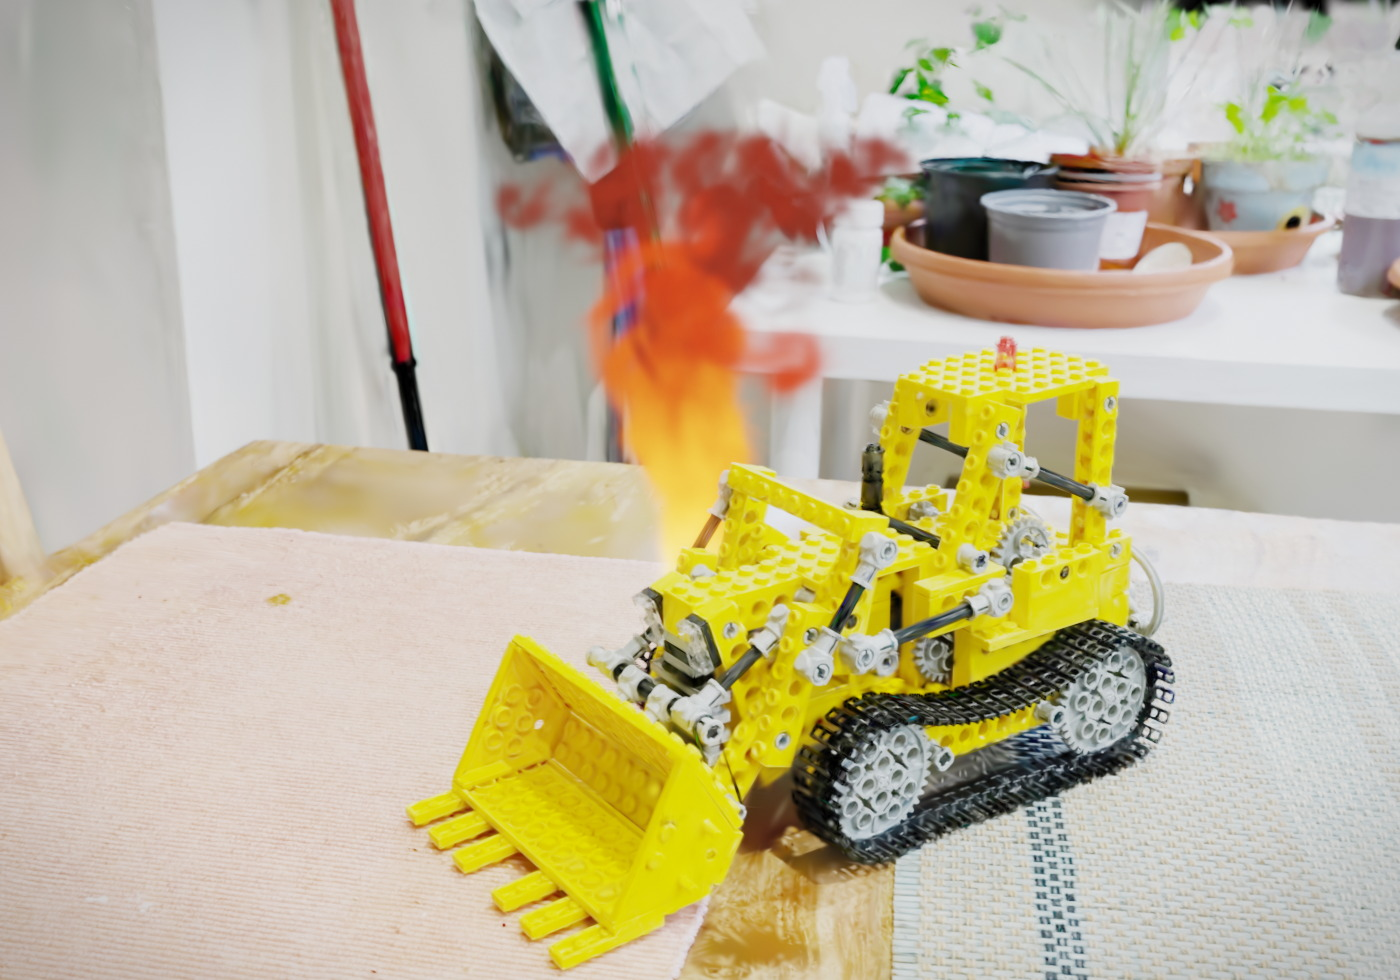
\includegraphics[width=.492\linewidth]{kitchen_ours}\hfill
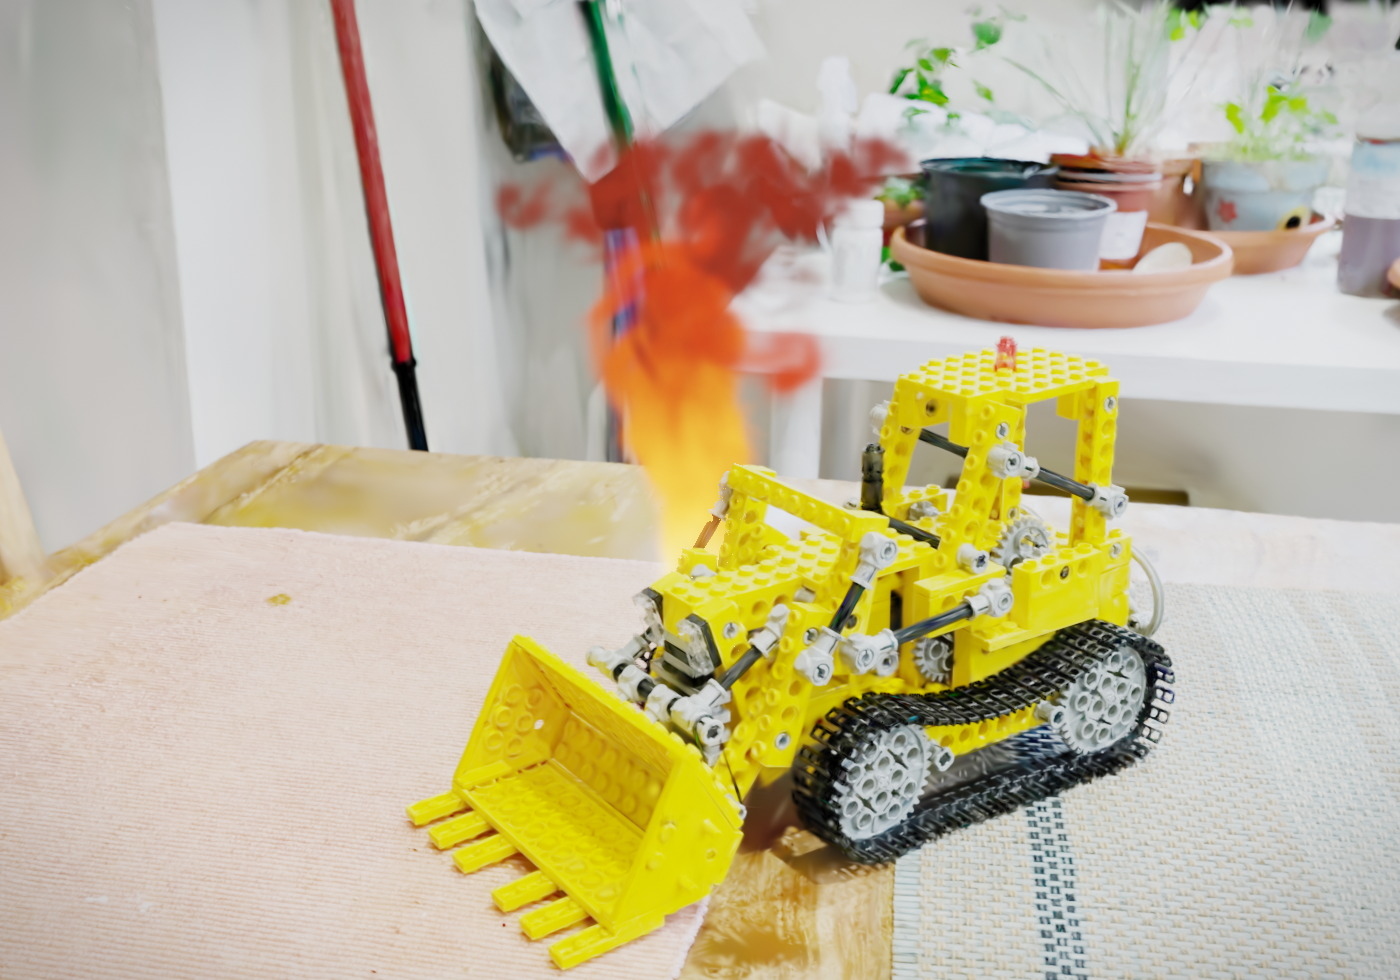
\includegraphics[width=.492\linewidth]{kitchen_depth}\\[2pt]
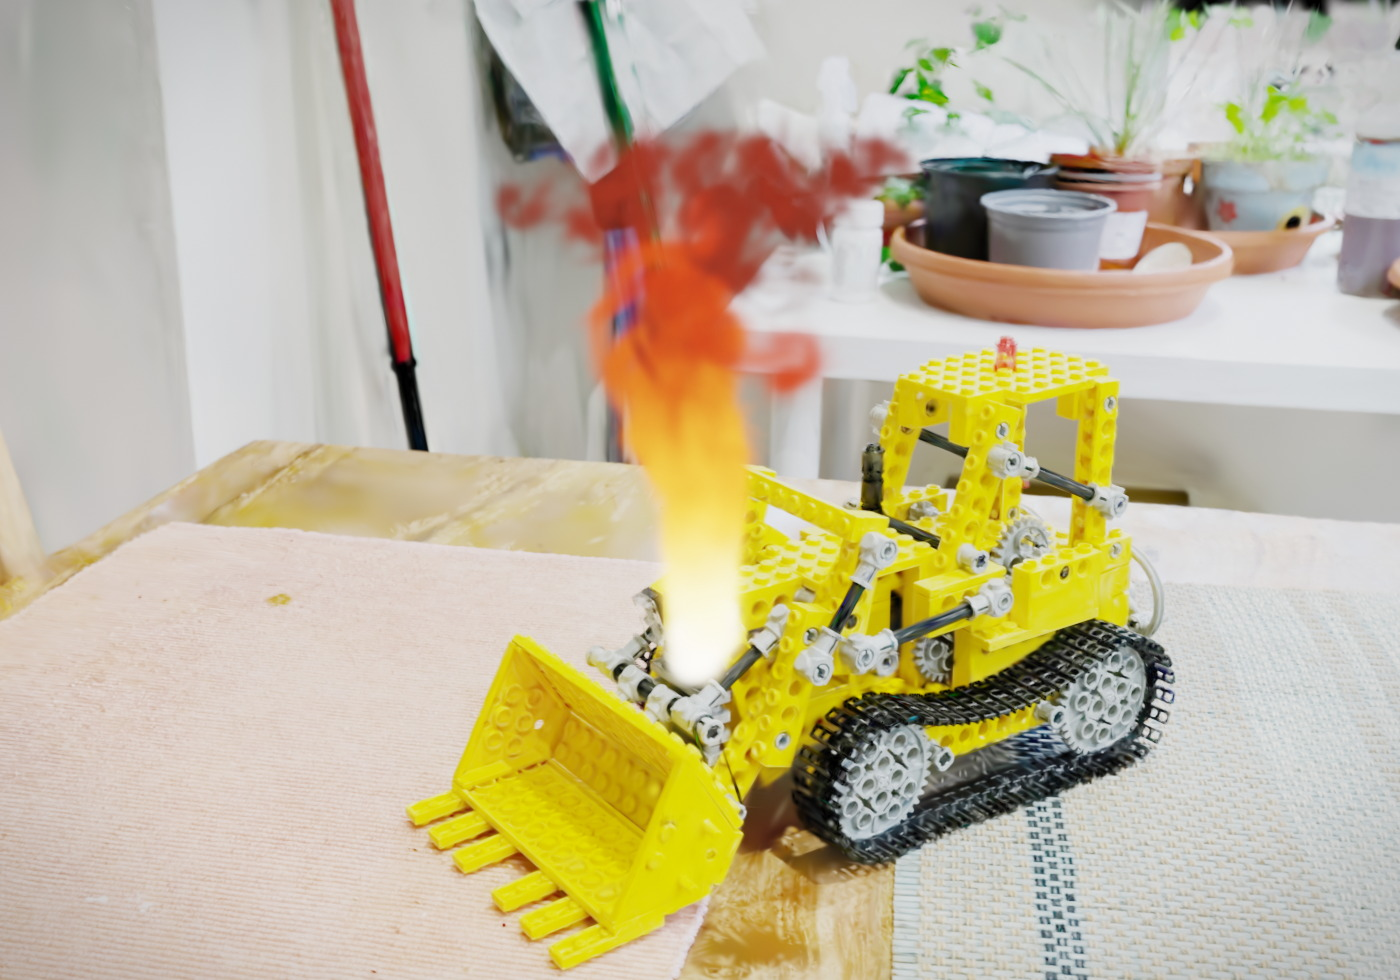
\includegraphics[width=.492\linewidth]{kitchen_backdrop}\hfill
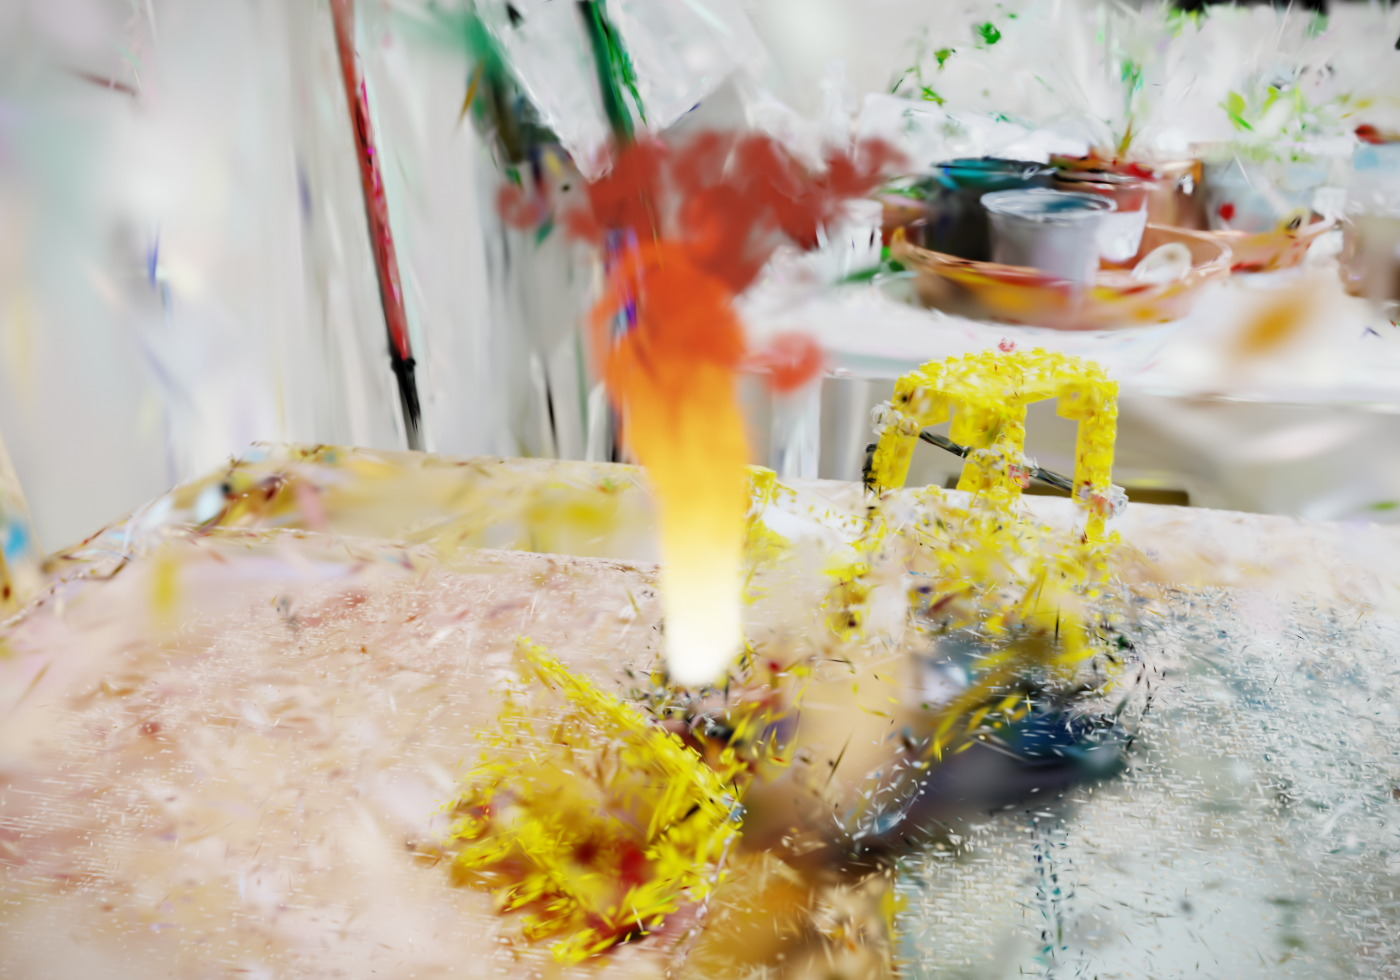
\includegraphics[width=.492\linewidth]{kitchen_unsorted}
\caption{The full \emph{kitchen} ladder. Top: ours (100\%), depth-aware (100.4\%). Bottom: backdrop (119.3\%), and backdrop with the intra-scene sort removed (112.8\%).}
\end{figure}

\begin{table}
\caption{Fire contribution of the depth-aware baseline relative to ours (\%), by opacity threshold.}
\footnotesize
\begin{tabular}{lrrrrrrrrr}
\toprule
$\alpha$ & .15 & .20 & .22 & .25 & .28 & .30 & .50 & .70 & .90 \\
\midrule
\emph{kitchen} & 99.9 & & & & & 100.1 & 100.4 & 101.4 & 110.2 \\
\emph{treehill} & 83.7 & 94.6 & 97.7 & 102.0 & 106.1 & 108.6 & 130.1 & 141.9 & 149.4 \\
\bottomrule
\end{tabular}
\end{table}

On \emph{treehill} backdrop gives 150.9\% and unsorted 153.0\%. The baseline's partial fraction is 9.3, 8.4, 5.1, 2.8, 0.6\% at $\alpha=0.15,0.30,0.50,0.70,0.90$. At the energy-matched point silhouette MAE is 16.5/255, and 91--95\% of silhouette pixels differ from ours by at least 3/255 at every threshold. Our transmittance histogram across ten equal bins is 3.1, 6.2, 8.3, 7.4, 8.1, 10.3, 10.5, 13.7, 13.2, 19.4\%. The white-hot core saturates over 14.3\% of the silhouette; excluding clipped pixels moves ours $88.1\to96.6$\%. Sweeping the silhouette threshold from 3 to 40 leaves ours at 82.0--88.1\% against 2.8--5.1\% at $\alpha=0.50$. The offline instrument on the raw \texttt{.ply} predicts 93.9\% partial at mean 0.713 against the renderer's 88.1\% and 0.616; the gap is expected, since that probe places the flame on one median depth plane.

The synthetic scene agrees with \emph{kitchen}: ours 100\%, depth-aware 101.8--107.9\% across the same thresholds, backdrop 117.9\%, unsorted 121.7\%; over the silhouette 86.0\% fully transmitted, 11.8\% blocked, 2.2\% partial.

\section{Renderer calibration}
Our rasterizer, in a plain mode with no bloom, tone styling or fire, draws the prepared \emph{kitchen} \texttt{.ply} at a fixed camera and $1400\times980$; gsplat 1.5.2 rasterizes the identical file at the identical camera. The two agree to 38.67\,dB (MAE 0.0051 in $[0,1]$). This is an equality test between forward rasterizers on one file. To show the loader introduces no error, gsplat is driven through our \texttt{.ply} parser against the real photographs at the released COLMAP poses on the uncropped release: 32.76\,dB, SSIM 0.951 over 21 training views, and 29.88\,dB, SSIM 0.917 over 3 held-out views at half resolution. These sit near published 3DGS figures for the scene. We claim nothing about the prepared asset's fidelity to the photographs, since the crop deletes room content.

\section{Interleave bound and overhead}
We built an order-exact reference, a single merge of the two streams by primitive depth, and measured the bucketed path against it over four cameras and $K$ from 24 to 65\,536, 60 runs in all. The largest out-of-order depth is 0.999961 of a bucket width and never reaches one. Inverted cross-stream pairs fall with exponents $-0.989$ to $-1.011$. At $K=1536$ the interleave alone reproduces the reference to 63.3--79.3\,dB (MAE 0.0007--0.008 of one 8-bit level); with the scene's own counting sort as shipped, 49.2--65.1\,dB. Buckets are uniform in linear view-space depth and share one key with the dynamic stream. On \emph{kitchen} the reconstruction spans 39.5 view-depth units, a bucket is 0.026 wide, and the flame occupies buckets 616--677.

Median render time with interleave against a draw-after pass is 22.9 vs.\ 21.2\,ms at 45.8k scene splats (+8\%, 38\,ns per splat) and 291.0 vs.\ 239.3\,ms at 729\,826 (+22\%, 71\,ns per splat). The premium is dominated by per-splat scatter into bucket order rather than by $K$: $K=96,384,1536,4096$ gives 22.7, 22.7, 22.9, 23.4\,ms at 45.8k, and $K=96$ vs.\ 1536 gives 284.4 vs.\ 291.0\,ms at 729\,826.

\section{Combustion runs}
\begin{figure*}
\centering
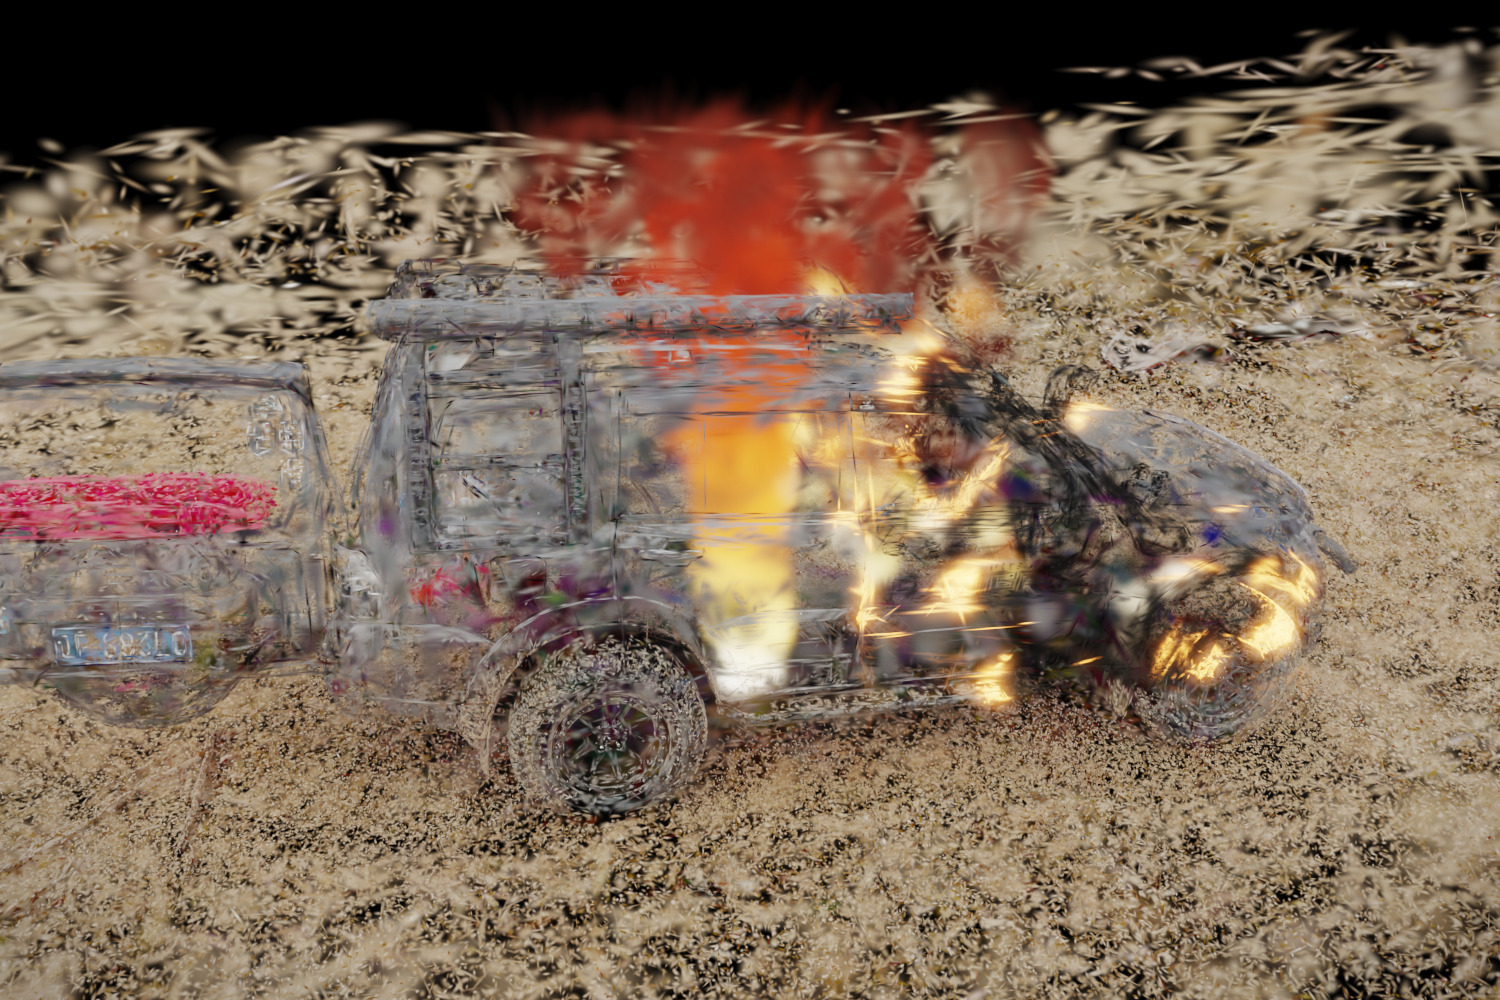
\includegraphics[width=.33\textwidth]{campsite_a}\hfill
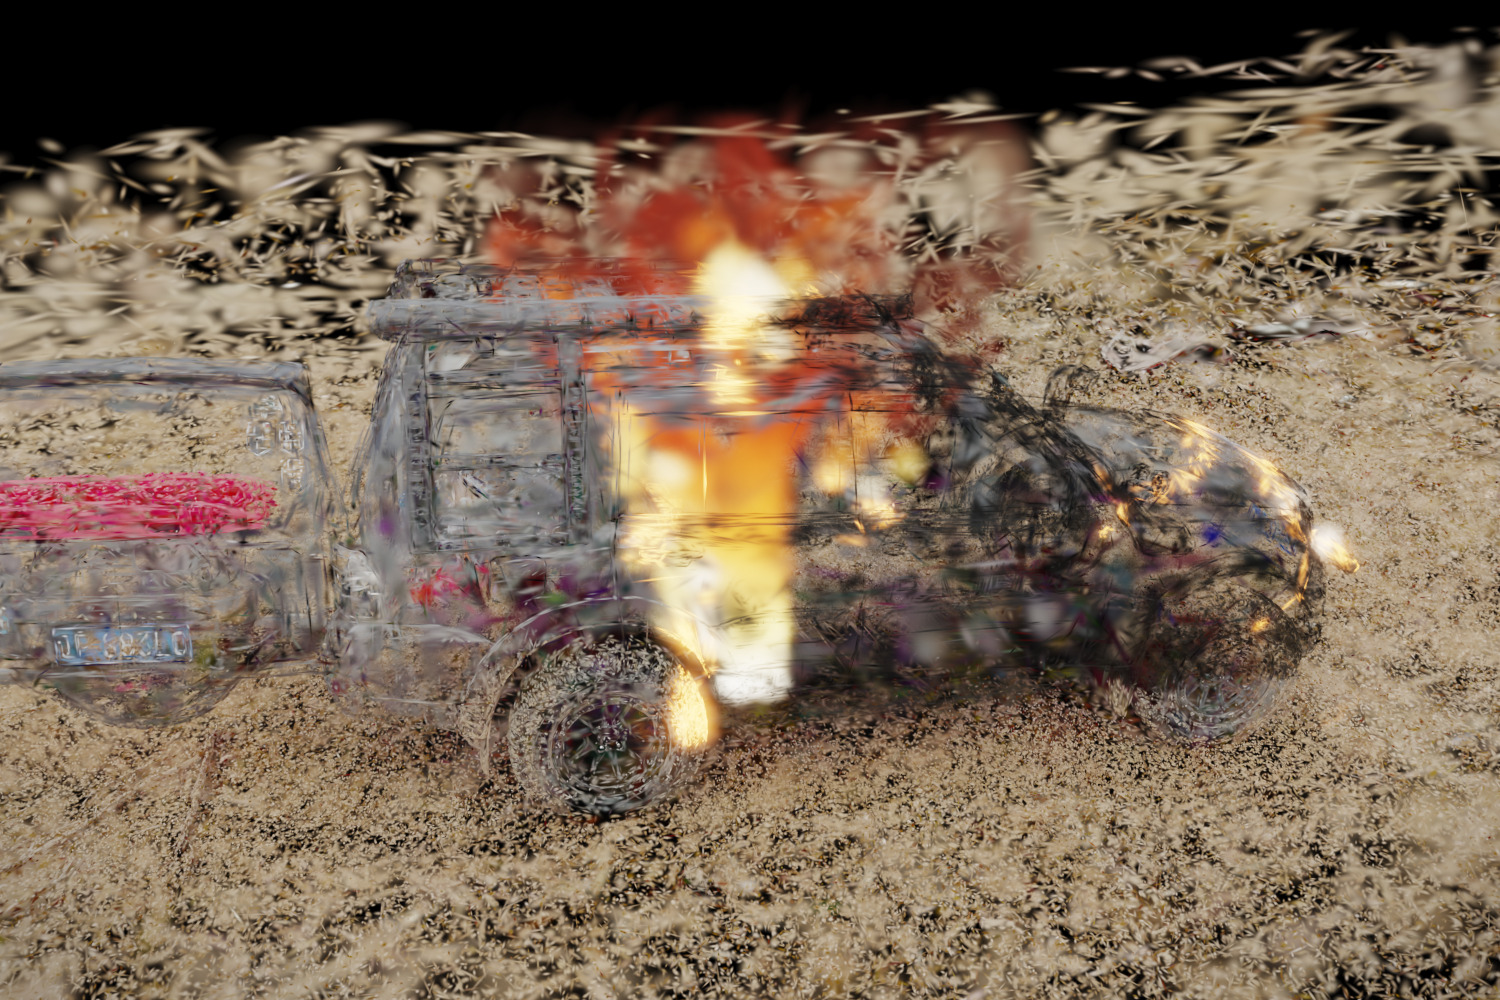
\includegraphics[width=.33\textwidth]{campsite_b}\hfill
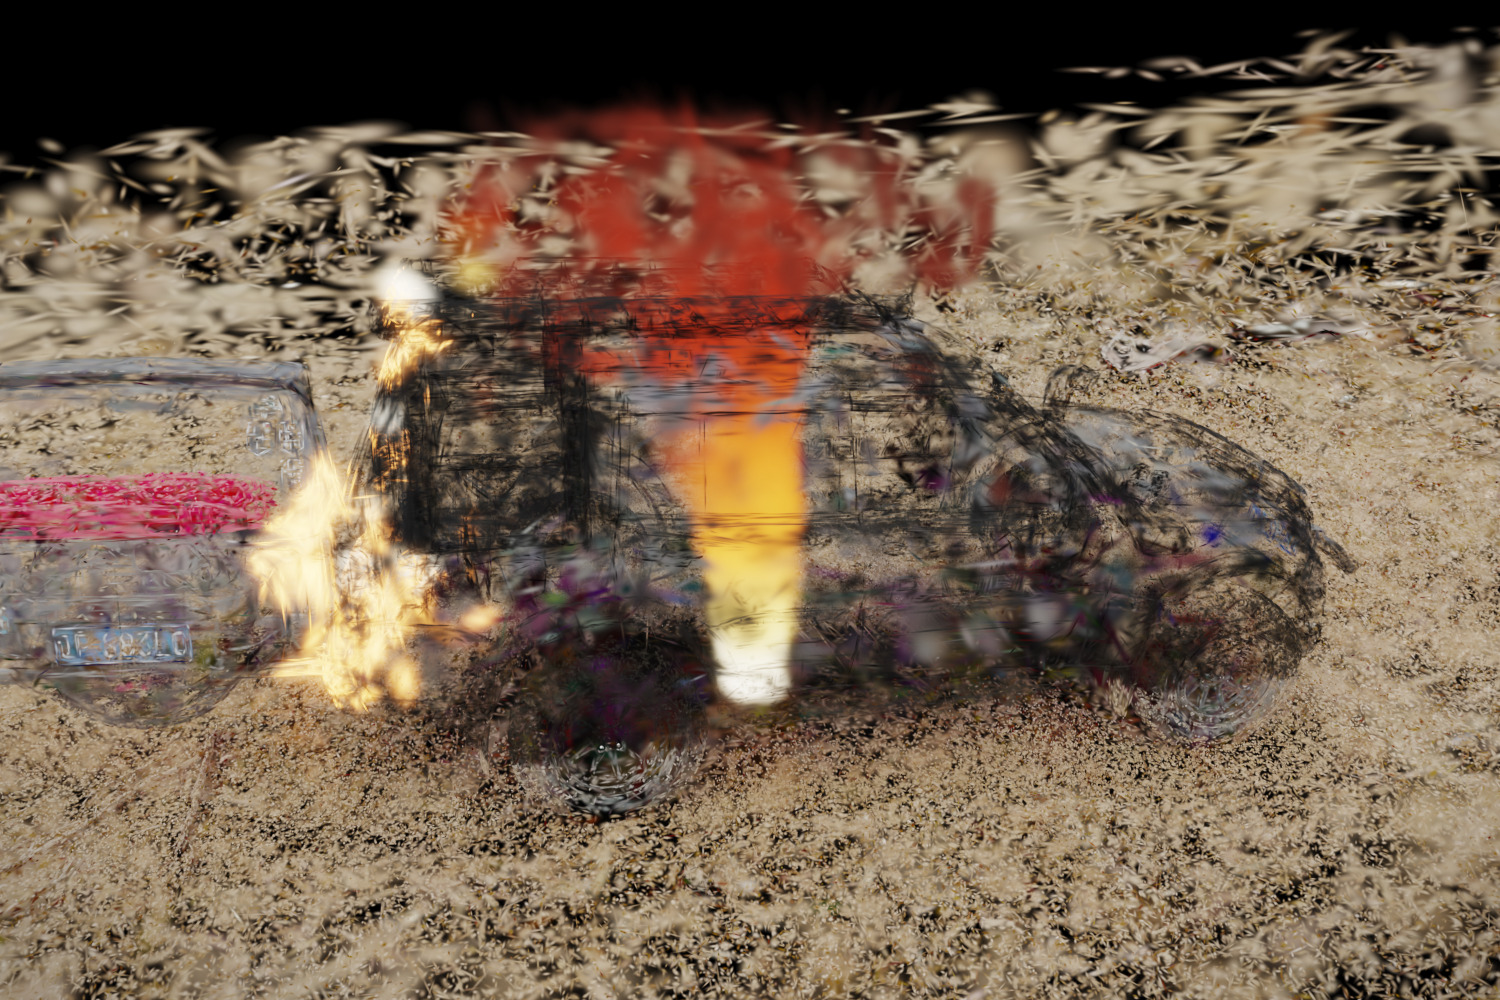
\includegraphics[width=.33\textwidth]{campsite_c}\\[2pt]
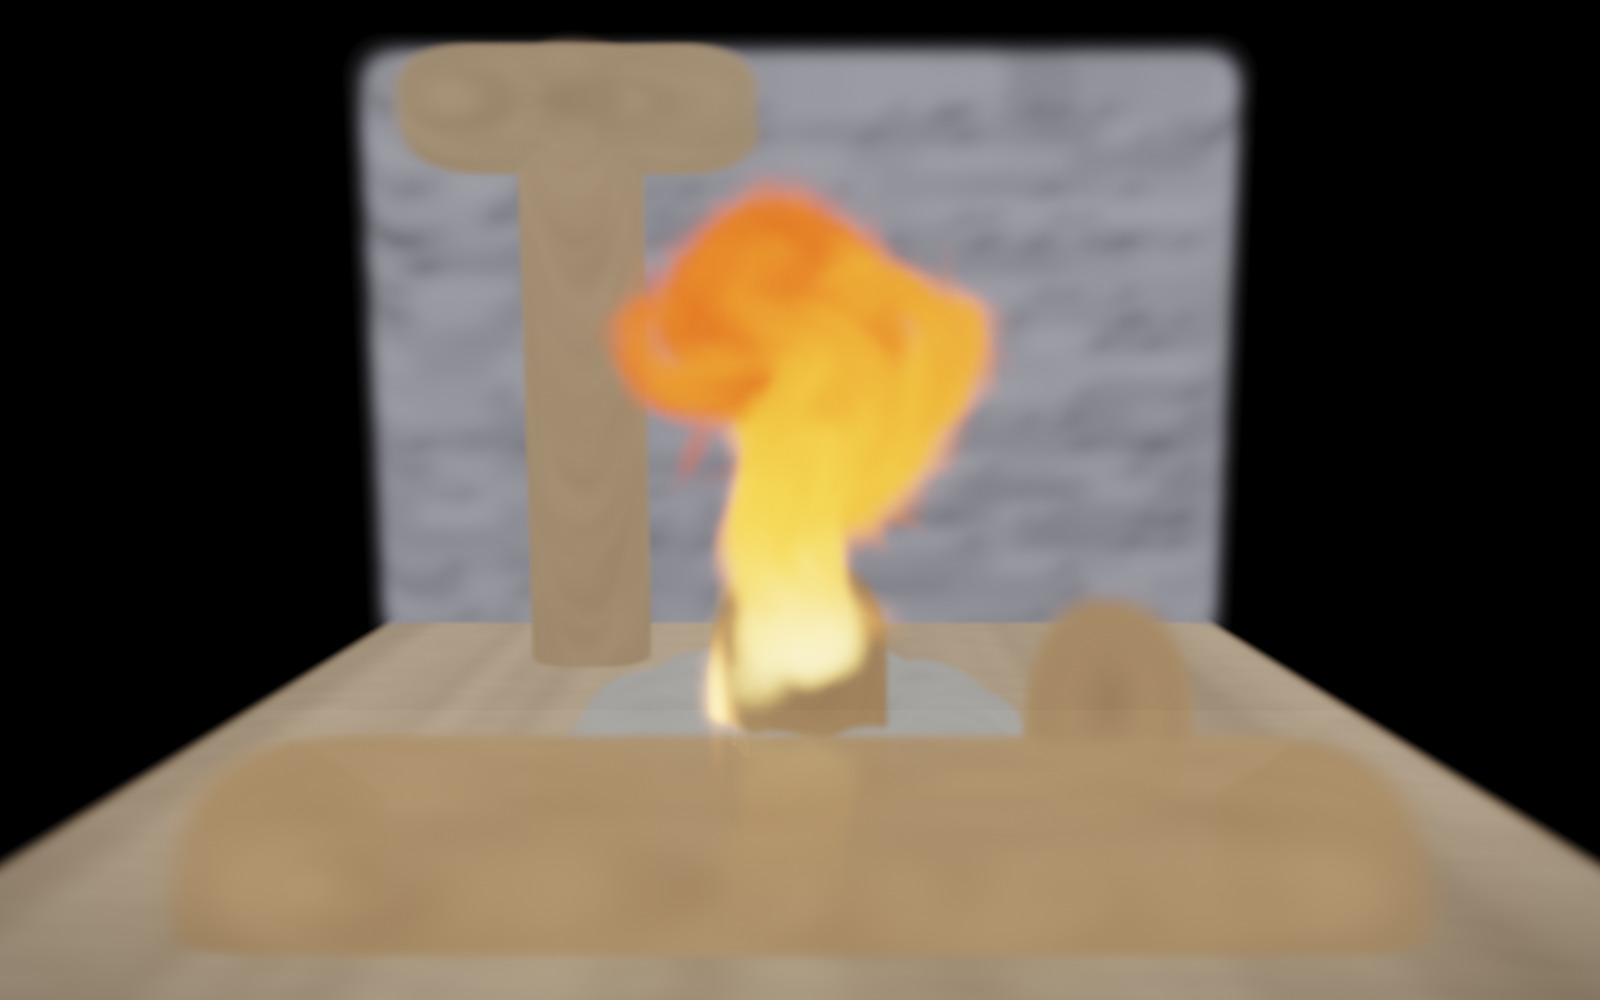
\includegraphics[width=.33\textwidth]{spread_a}\hfill
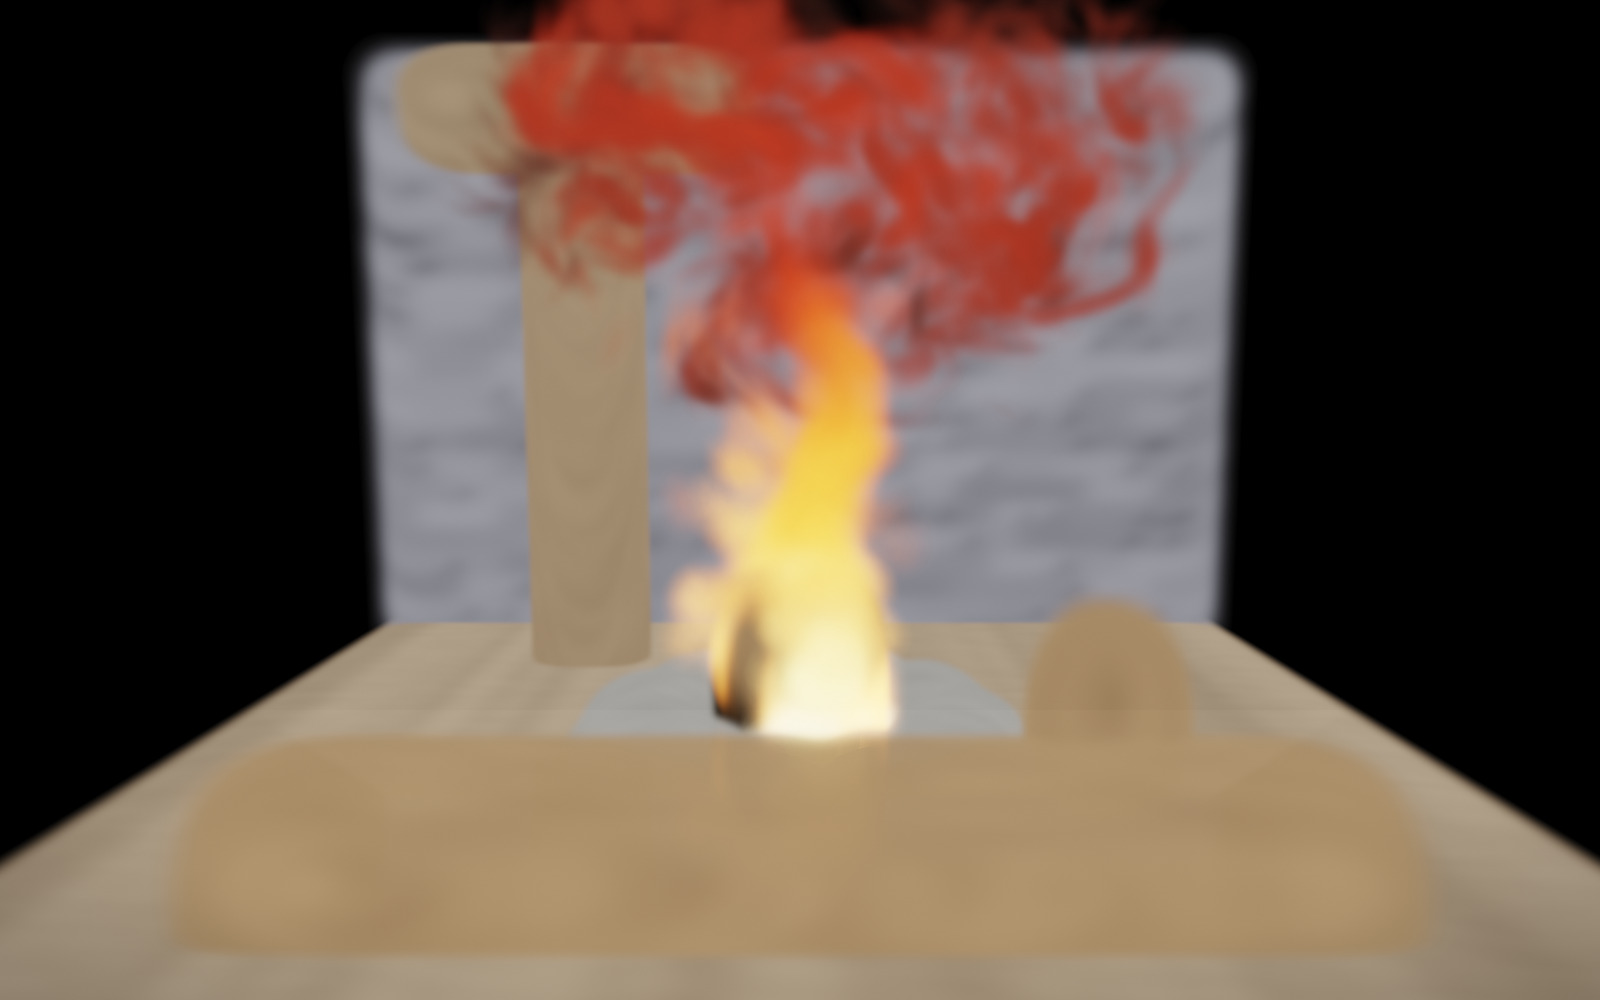
\includegraphics[width=.33\textwidth]{spread_b}\hfill
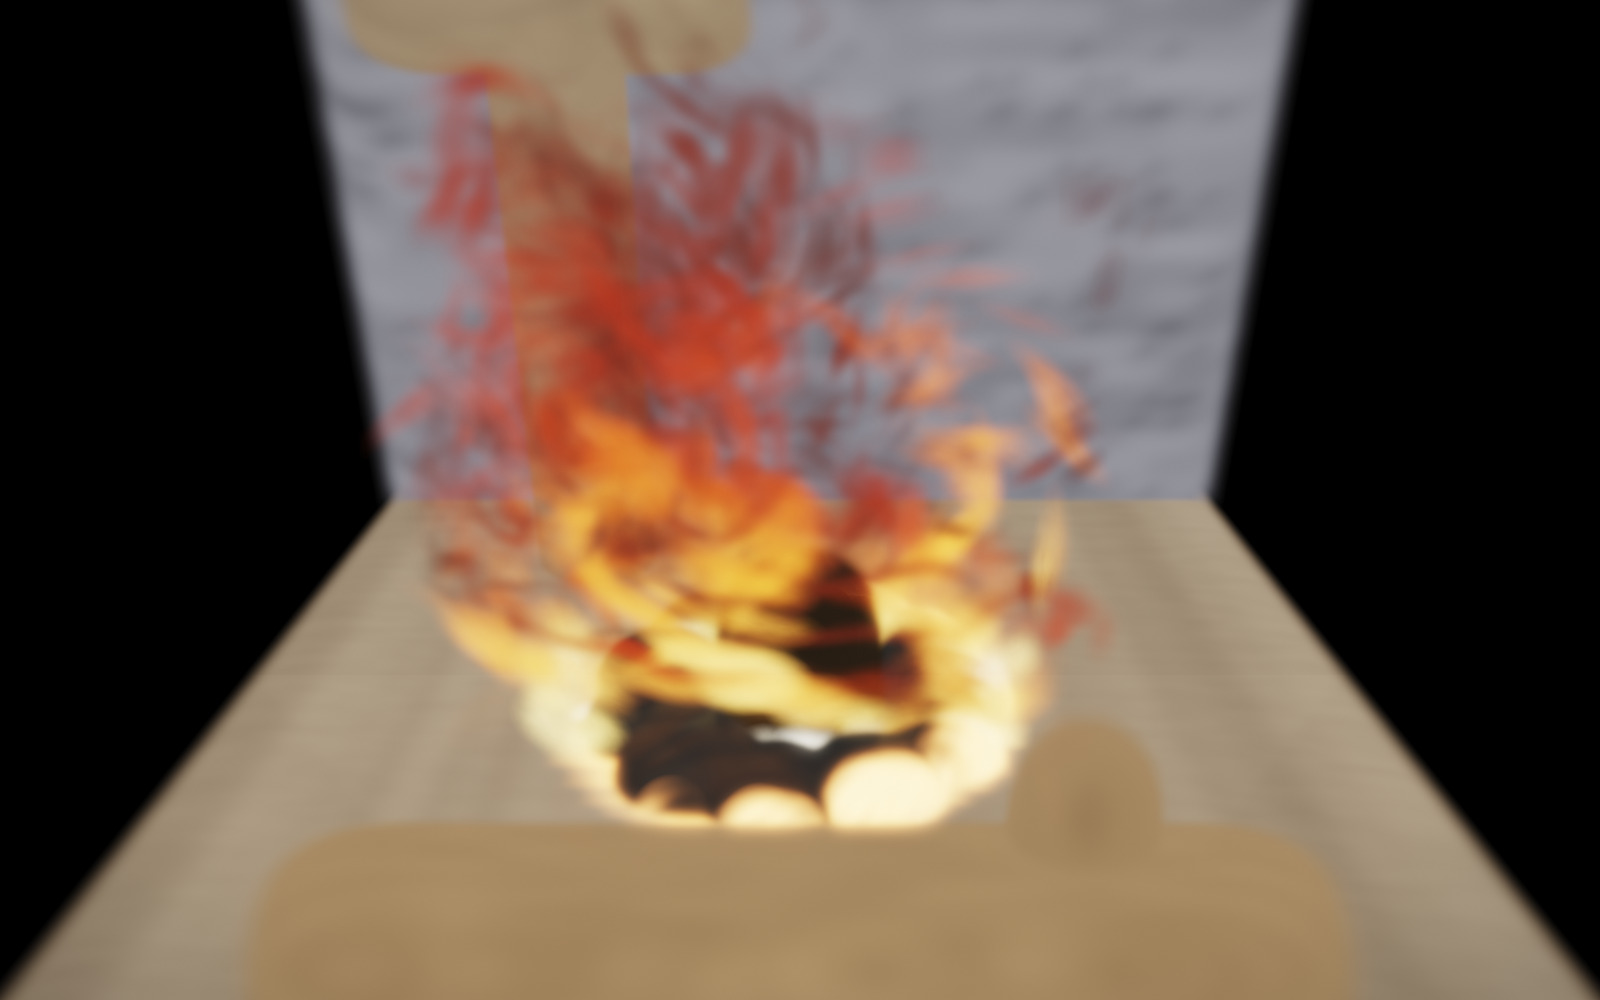
\includegraphics[width=.33\textwidth]{spread_c}
\caption{Top: the loop on the campsite capture. Fuel is a $5.0\times1.7\times2.1$\,m box, 44\,861 of 380\,000 splats, with a single ignition of 40 splats. At $t=35,85,165$ steps: 2\,591 burning and 7\,000 charred; 2\,068 and 18\,392; 1\,611 and 37\,800. Bottom: the loop on the synthetic scene from a single ignition of 4\,083 splats, at $t\approx2,16,56$\,s; 12\,600 charred at the end.}
\end{figure*}

\paragraph{Budgets and cost.} Per frame the loop uses at most 160 flame-particle heat samples, 48 seed emissions and 1\,400 frontier splats. Disabling the loop costs 31\,ms per substep on the campsite and 32\,ms on \emph{kitchen}; enabling it with nothing burning costs 33\,ms on both, so the $O(n)$ decay scan is $\sim$2\,ms. With $\sim$2.5k splats burning a substep is 99\,ms on the campsite, the frontier alone 66\,ms at 27\,$\mu$s per burning splat, and 146\,ms on \emph{kitchen} with $\sim$2.8k burning at 41\,$\mu$s per splat. On the campsite a query that returns 81 true neighbours scans 405 candidates through the adjacency hash.

\paragraph{\emph{kitchen} run.} Fuel boxes in the demo's world frame: the machine $x\in[0.28,2.90]$, $y\in[0.095,2.20]$, $z\in[-2.15,1.70]$ (75\,443 splats) and the strip $x\in[-1.60,3.20]$, $y\in[0.00,0.12]$, $z\in[-1.30,0.45]$ (25\,430 splats, 260 shared). The selection was checked by rendering the subset and its complement, and 26-connected labelling puts 73\,346 of 75\,443 in one component. The blade teeth stay unburnt because they lie below the box's floor, which the tabletop plane forces; lowering it sweeps in 47\,002 table splats to gain $\sim$1k machine ones. Lit machine splats: 170 at $t=40$\,s, 1\,039 at 60, 9\,389 at 100, 21\,934 at 150, 35\,893 at 200, 48\,757 at 249.73. Charring accumulates at 210--245 splats per simulated second, set by the frontier cap, while the frontier stands at 1\,893--8\,041 splats. The run took 15\,044 substeps and $\sim$45 minutes.

\paragraph{Gap crossing.} On the synthetic scene ignition did not cross fuel gaps of 0.12--0.65 world units ($1.1$--$6\times$ the adjacency radius) in 35 simulated seconds at winds up to $2\times$ default, because hot particles rise at $\sim$1.1 units/s against a lateral 0.35--0.6. On \emph{kitchen} the fuel is continuous, so what crosses is the splat graph rather than the flame. Embers are visual only.

\paragraph{Char operator.} Over the 11\,522 most deeply charred pixels, an opacity drop moves composited colour by under 1/255, so the visual outcome is set by the albedo operator. A multiply preserves linear chromaticity and pushes colour back into the linear part of the tone curve, and measured saturation rises $0.513\to0.640$. Our operator gives 0.141. Luminance gradient holds at $0.78\times$ the uncharred render against $0.85\times$ for the multiply, while mixing straight to a flat soot albedo collapses it to $0.39\times$.

\section{Spectral protocol and controls}
\begin{figure}
\centering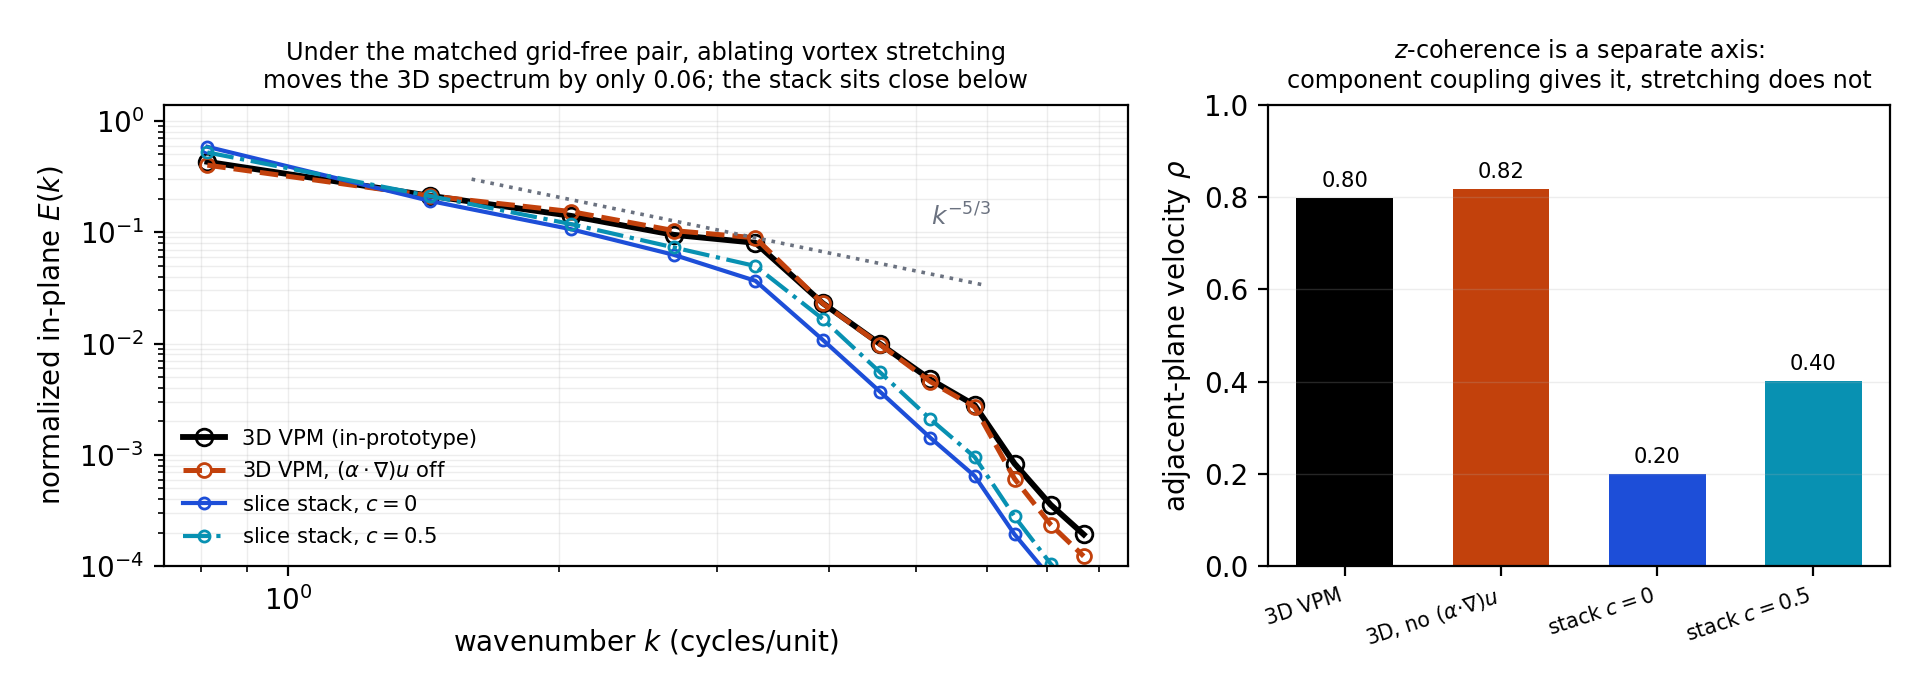
\includegraphics[width=\linewidth]{stretching}
\caption{Ablating vortex stretching inside the matched 3D solver. The bars at right are single-run values; four-seed means for the stack are 0.18 uncoupled and 0.29 coupled, as quoted in the main text.}
\end{figure}

\paragraph{Protocol.} The reference is a $32\times48\times32$ Boussinesq Euler solve with the same domain, cell size, heat source, cooling and $\Delta t$ as the stack, compared on the in-plane fluctuation field on planes at the nine slices' depths, 40 snapshots after warm-up. The stack is exported with procedural turbulence and wind disabled. Single-seed excursion from any mean is at most 0.035 in distance on the grid-free side. Kernel energy aliasing into the export is $\sim$4\% amplitude at the sampling Nyquist. The all-bin distance weights twelve bins equally, so 81--94\% of its grid-free value comes from six bins carrying 2.3\% of reference energy. Restricted to the other 97.7\%, distances are 0.05--0.26 against 0.66--0.87 for the grid-based stack; we quote the stricter all-bin figure in the main text.

\paragraph{Controls.} \emph{Density:} at 2600 per layer ($h/\sigz=0.25$) distance moves $0.46\to0.38$, largest bin 0.50, mid-band 0.28, toward the reference. \emph{Grid refinement:} at $64\times96$ the vortex-in-cell stack reaches 0.19 uncoupled and 0.41 coupled, with coherence 0.41 and cost 33.4\,ms at $9\times600$. \emph{Core radius:} at $\sigz=0.035$ distance drops to 0.16 with $\rho=0.61$ at no added cost; at $\sigz\geq0.07$ the field over-smooths (distance 1.5--2.3). \emph{Blur null:} a separable in-plane blur moves uncoupled $\rho$ from 0.181 to at most 0.225 while taking distance from 0.53 to 3.82. \emph{Timestep:} $\Delta t=1/30$ and $1/120$ move the distance by under 0.03 (0.59, 0.58, 0.55).

\paragraph{3D control.} The in-prototype 3D solver uses vector circulation with the erf-form regularized kernel \cite{winckelmans1993} and analytic stretching. It reproduces the external reference's character (largest bin 0.43 against 0.48, mid-band 0.34 against 0.30). Ablating stretching moves it to 0.40 and 0.37. Grid-based controls attribute $\sim$70\% of a four-times-larger gap to stretching, so the attribution is discretization-dependent. At matched budget its step is $2.8\times$ the stack's (27.5 vs.\ 9.9\,ms); a five-seed re-measurement gives $3.1\times$. At equal wall-clock cost, 215 vortons per slab reach distance 0.23 with $\rho=0.77$ and 1.9k renderable Gaussians.

\paragraph{Snapshot coherence probe.} Mean Pearson correlation of adjacent slices' velocity under the replay protocol (3 seeds, 4 snapshots, 600-frame warm-up, $c=0$) sits at 0.26--0.38 across $\kappa_z\in[0,1.2]$ with no significant trend, because shared source geometry dominates. The coherence claim therefore rests on the field-export protocol.

\section{Why we do not normalize across systems}
Published times place the design point: FieryGS at 2.37\,s per frame on an RTX 4090D, Gaussian Fluids at 38--228\,s per step on an RTX 4090, production layered fire at $\sim$20\,s per slice per frame. We do not divide them by a hardware factor. Peak FP32 and memory bandwidth rise by different ratios ($2.77\times$ and $1.33\times$ from RTX 3080 to 4090), our simulation runs on the CPU, and per-element normalization inverts the conclusion, since a grid cell and a Lamb--Oseen blob are not the same unit of work \cite{hoefler2015}. Only FieryGS addresses the same problem, with $\sim\!10^3\times$ our simulation state and unreported render resolution, so we compare architecture rather than wall clock. Within our system, rasterization is $\sim$0.37\,$\mu$s per scene Gaussian and throughput is $\sim$33.6M treecode interactions per second, single-threaded.

\section{Ablation figures}
\begin{figure}
\centering
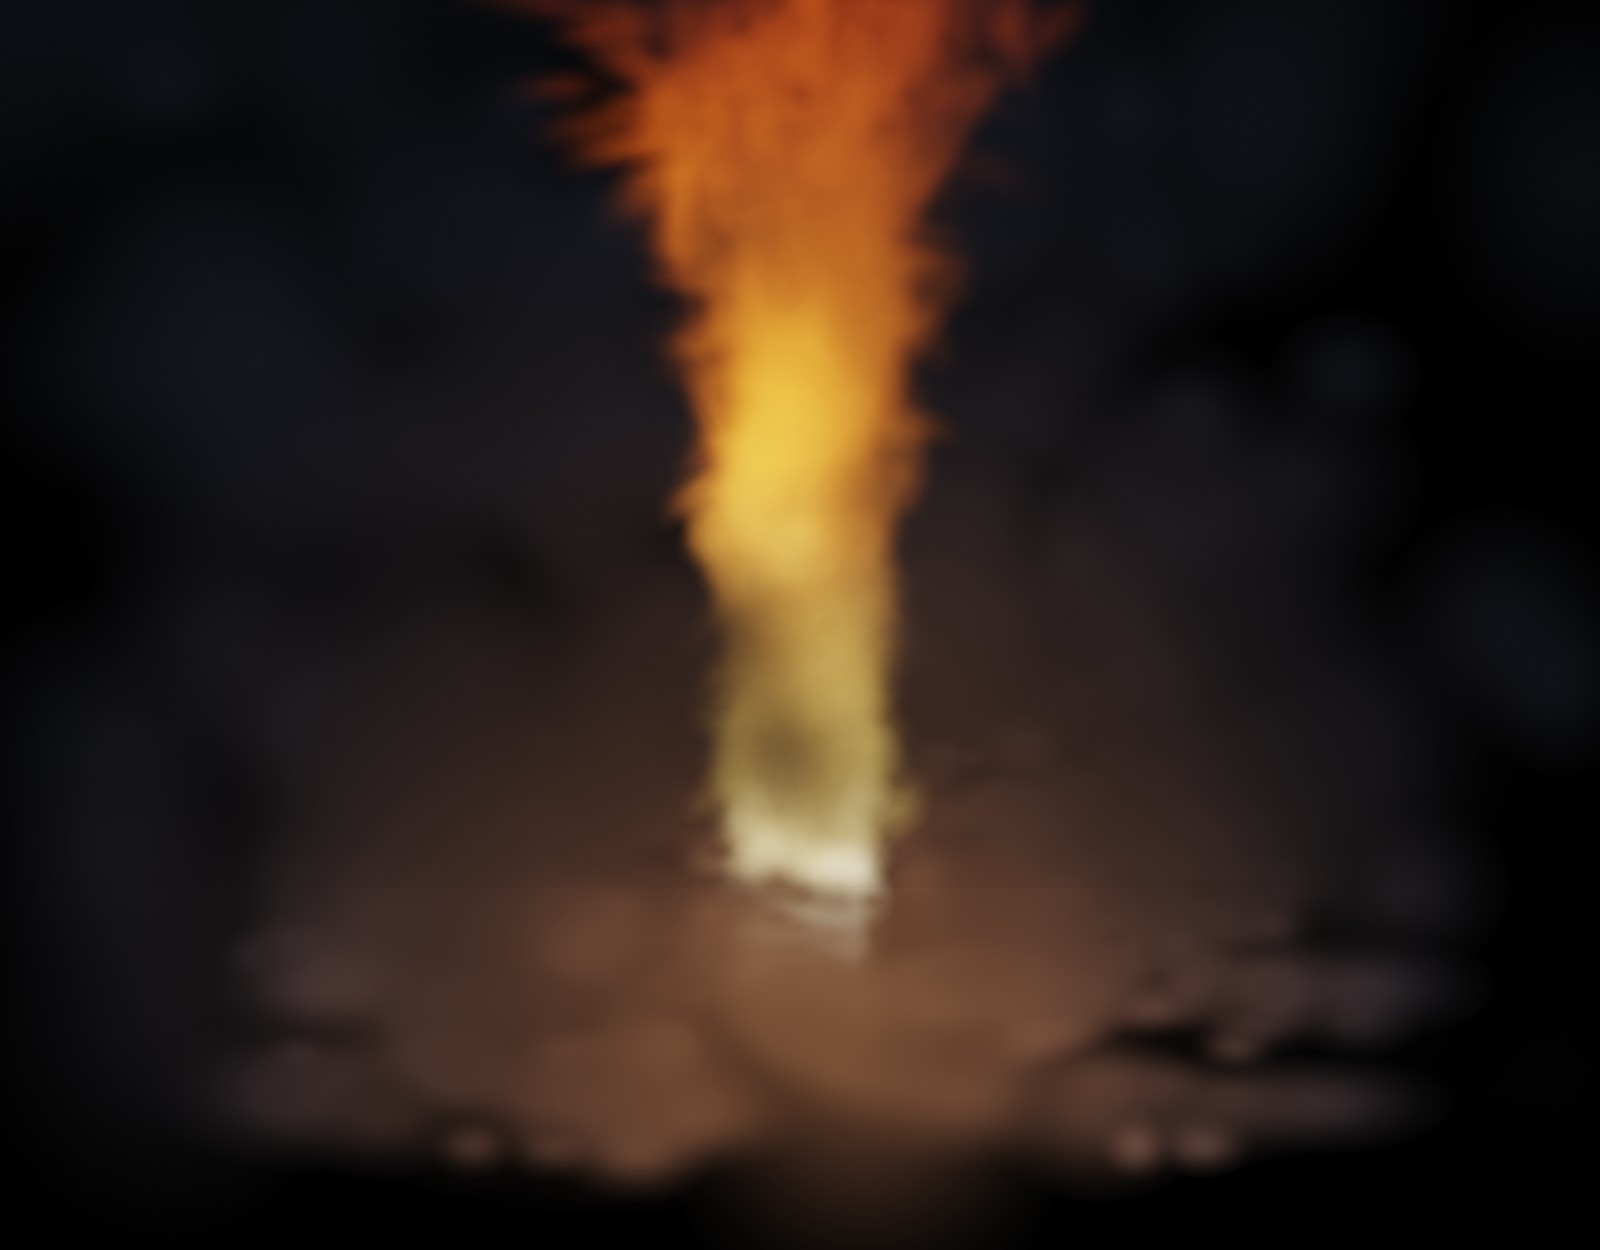
\includegraphics[width=.492\linewidth]{source_proc}\hfill
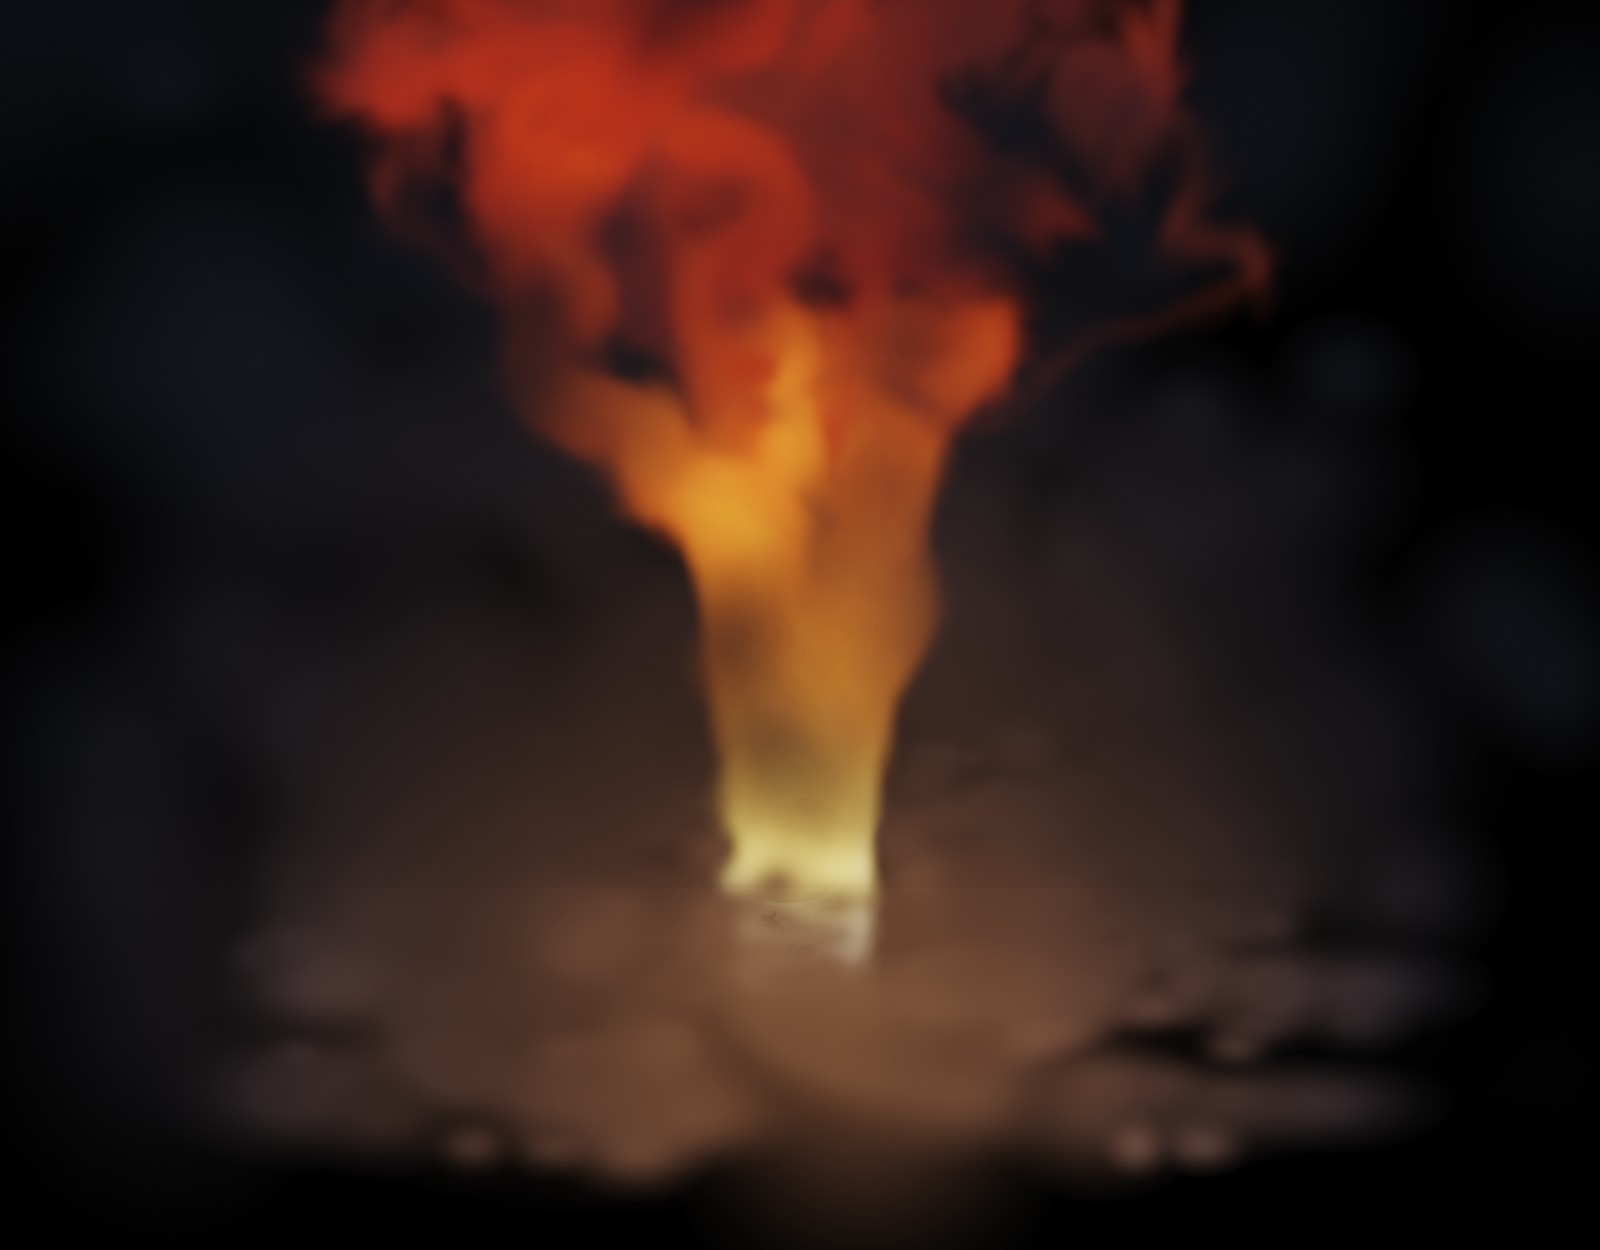
\includegraphics[width=.492\linewidth]{source_sim}\\[2pt]
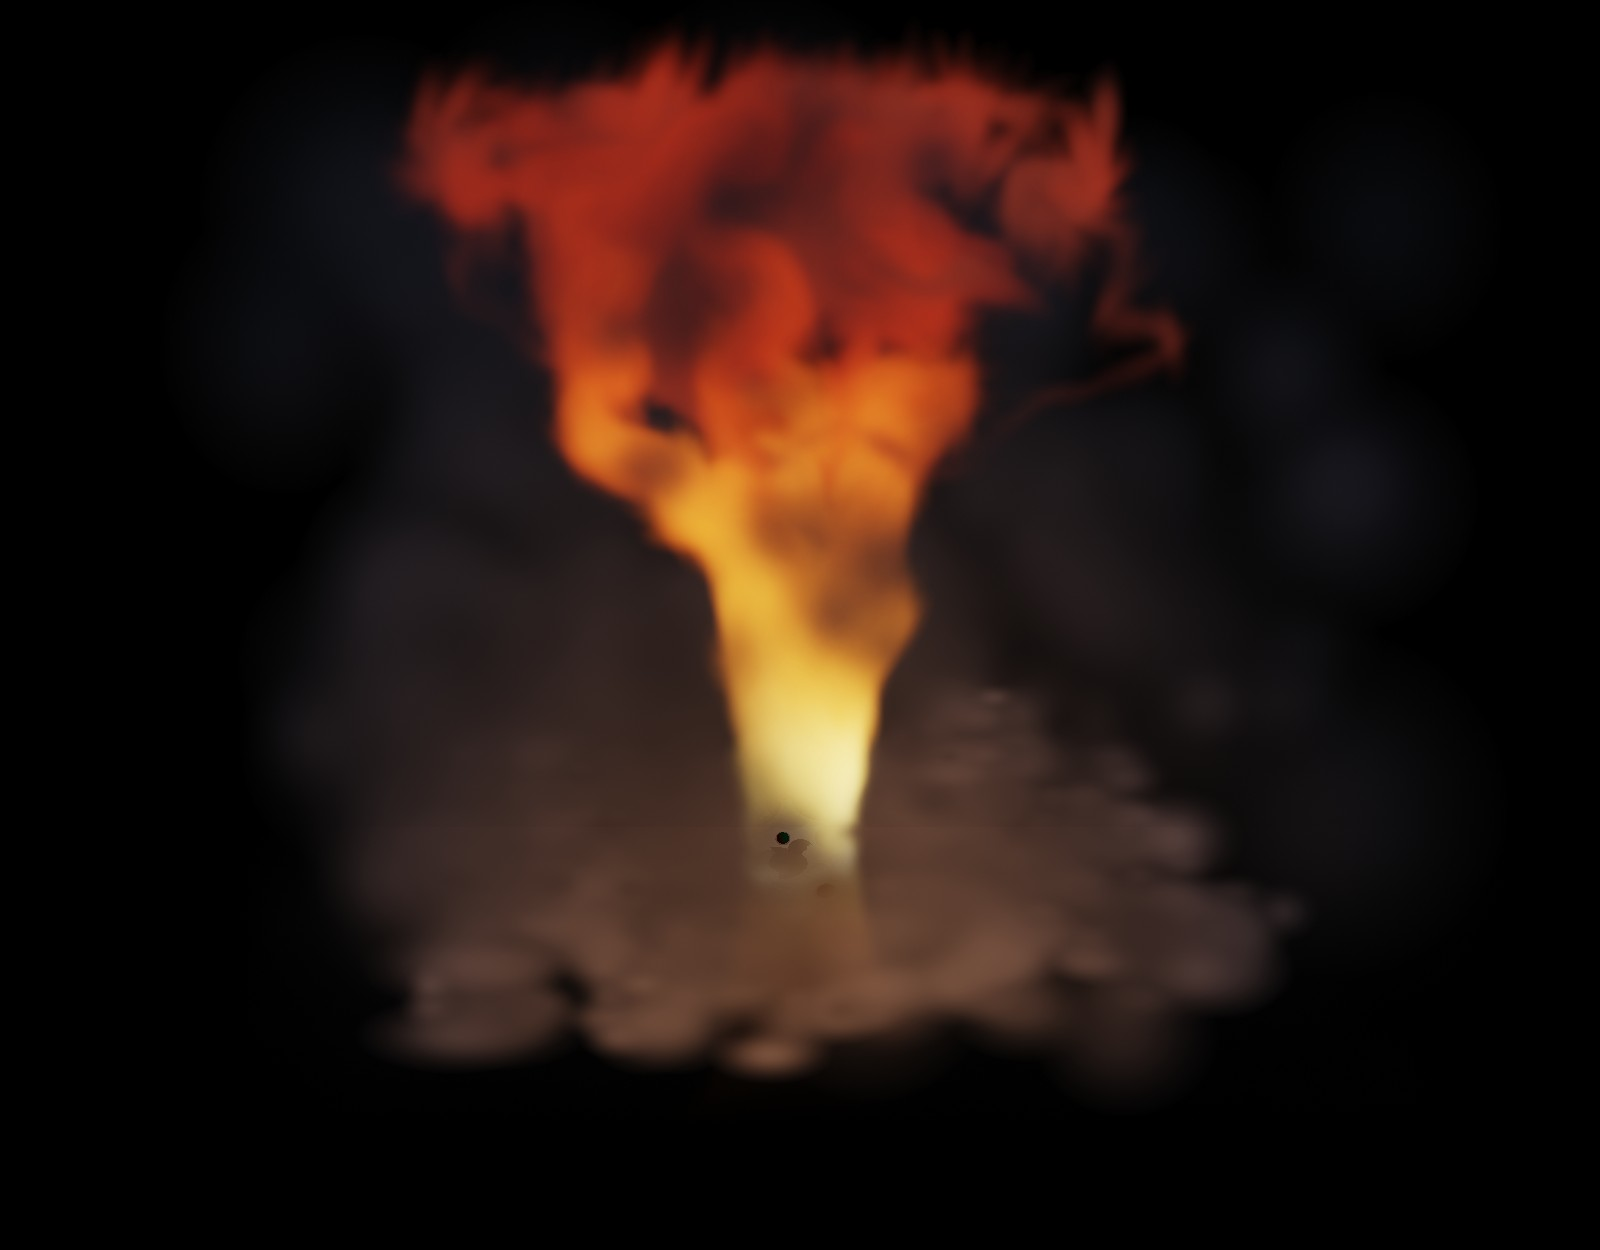
\includegraphics[width=.492\linewidth]{slice_view}\hfill
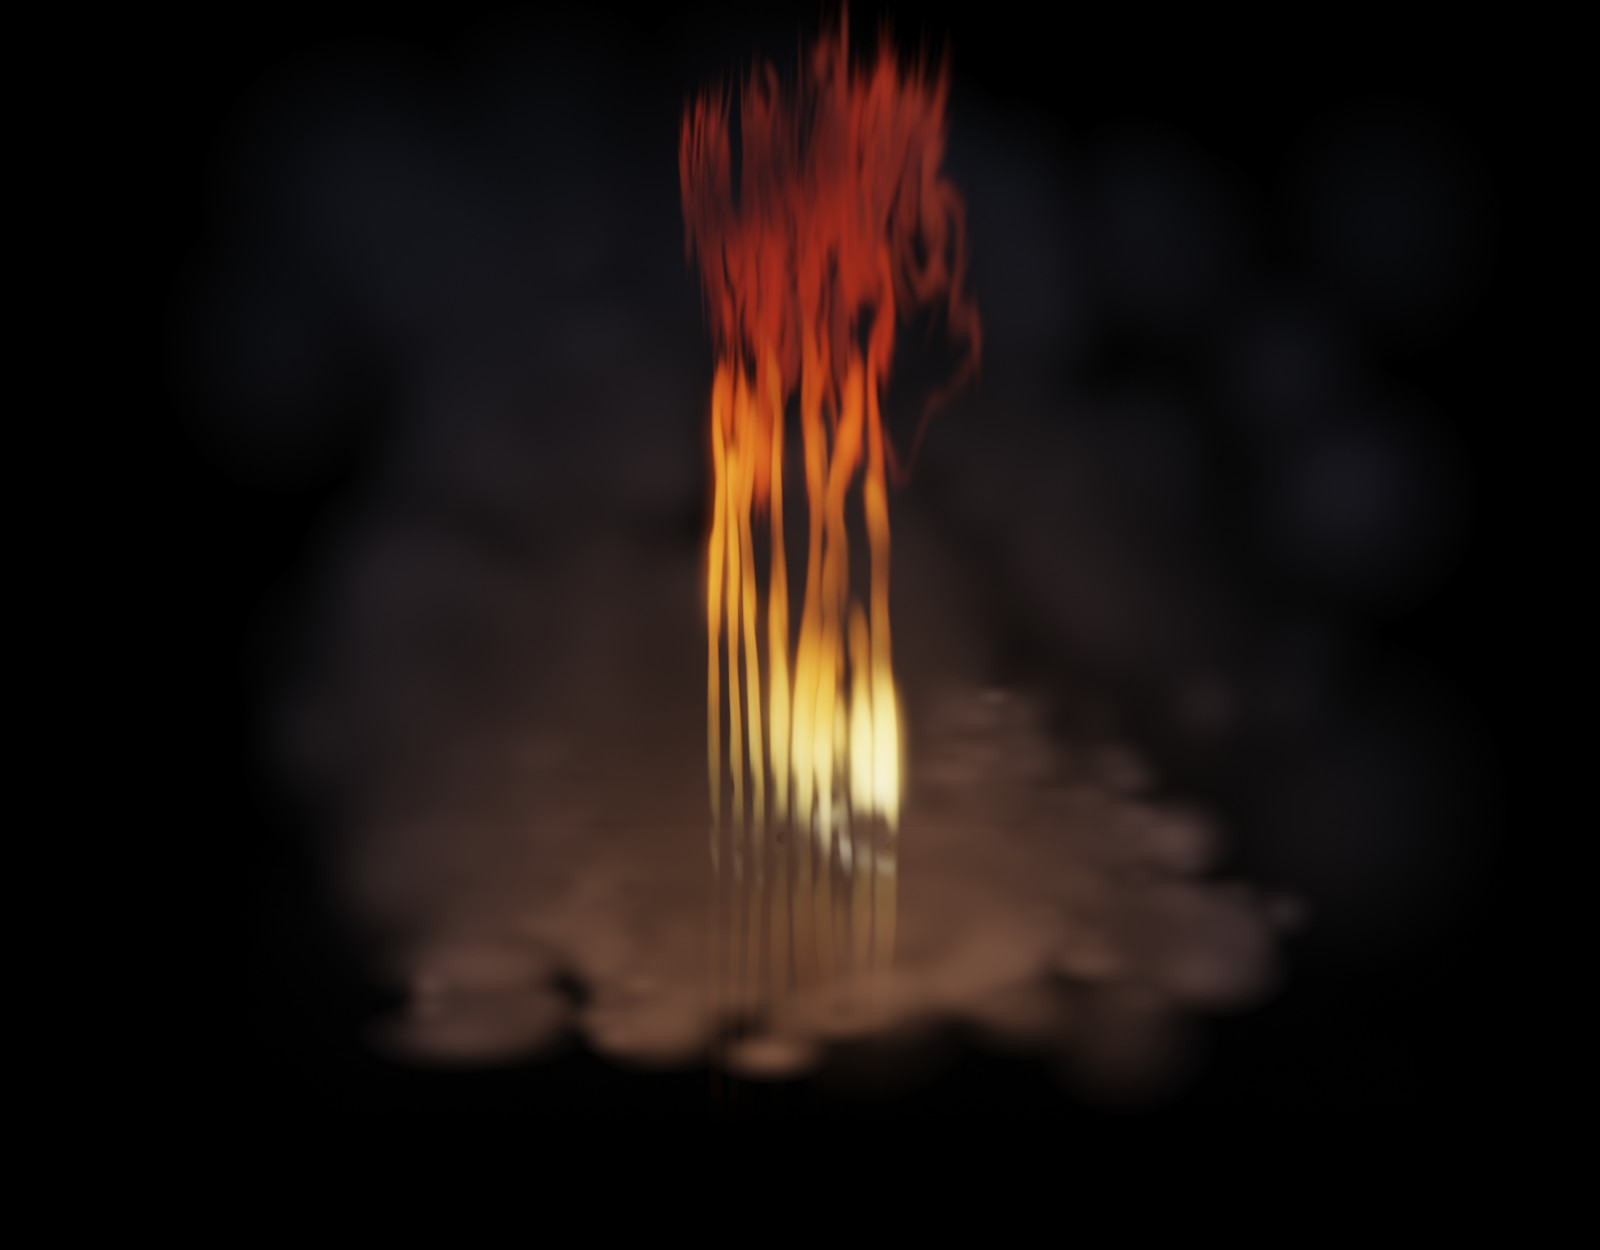
\includegraphics[width=.492\linewidth]{slice_world}\\[2pt]
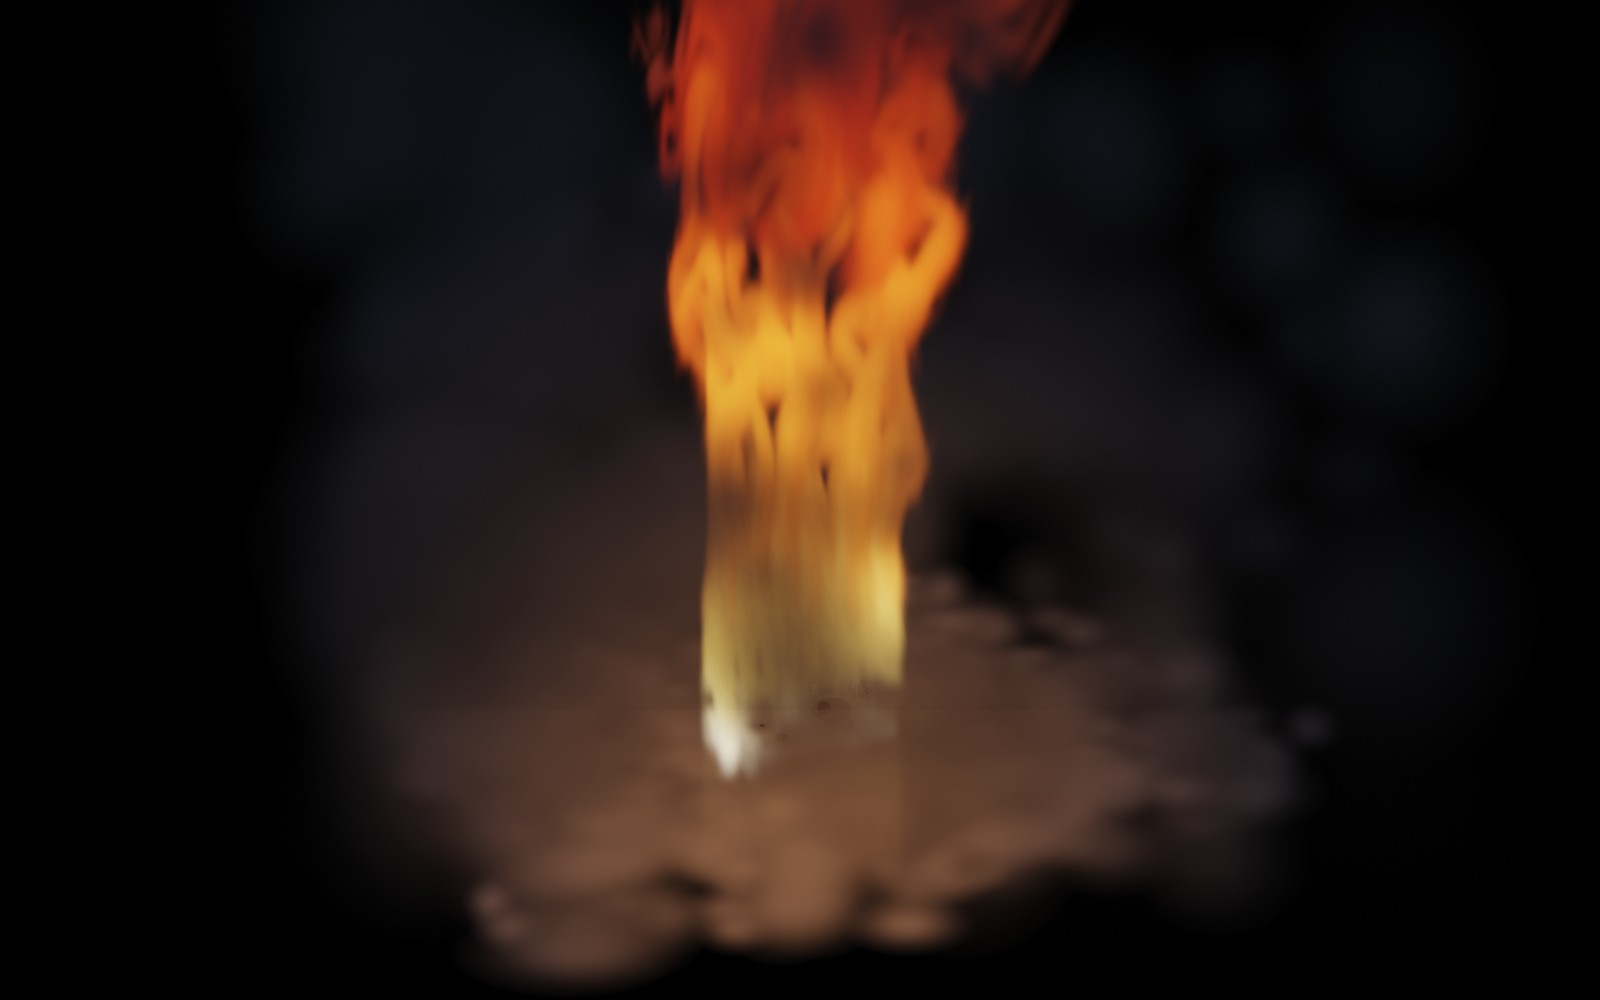
\includegraphics[width=.492\linewidth]{interz_off}\hfill
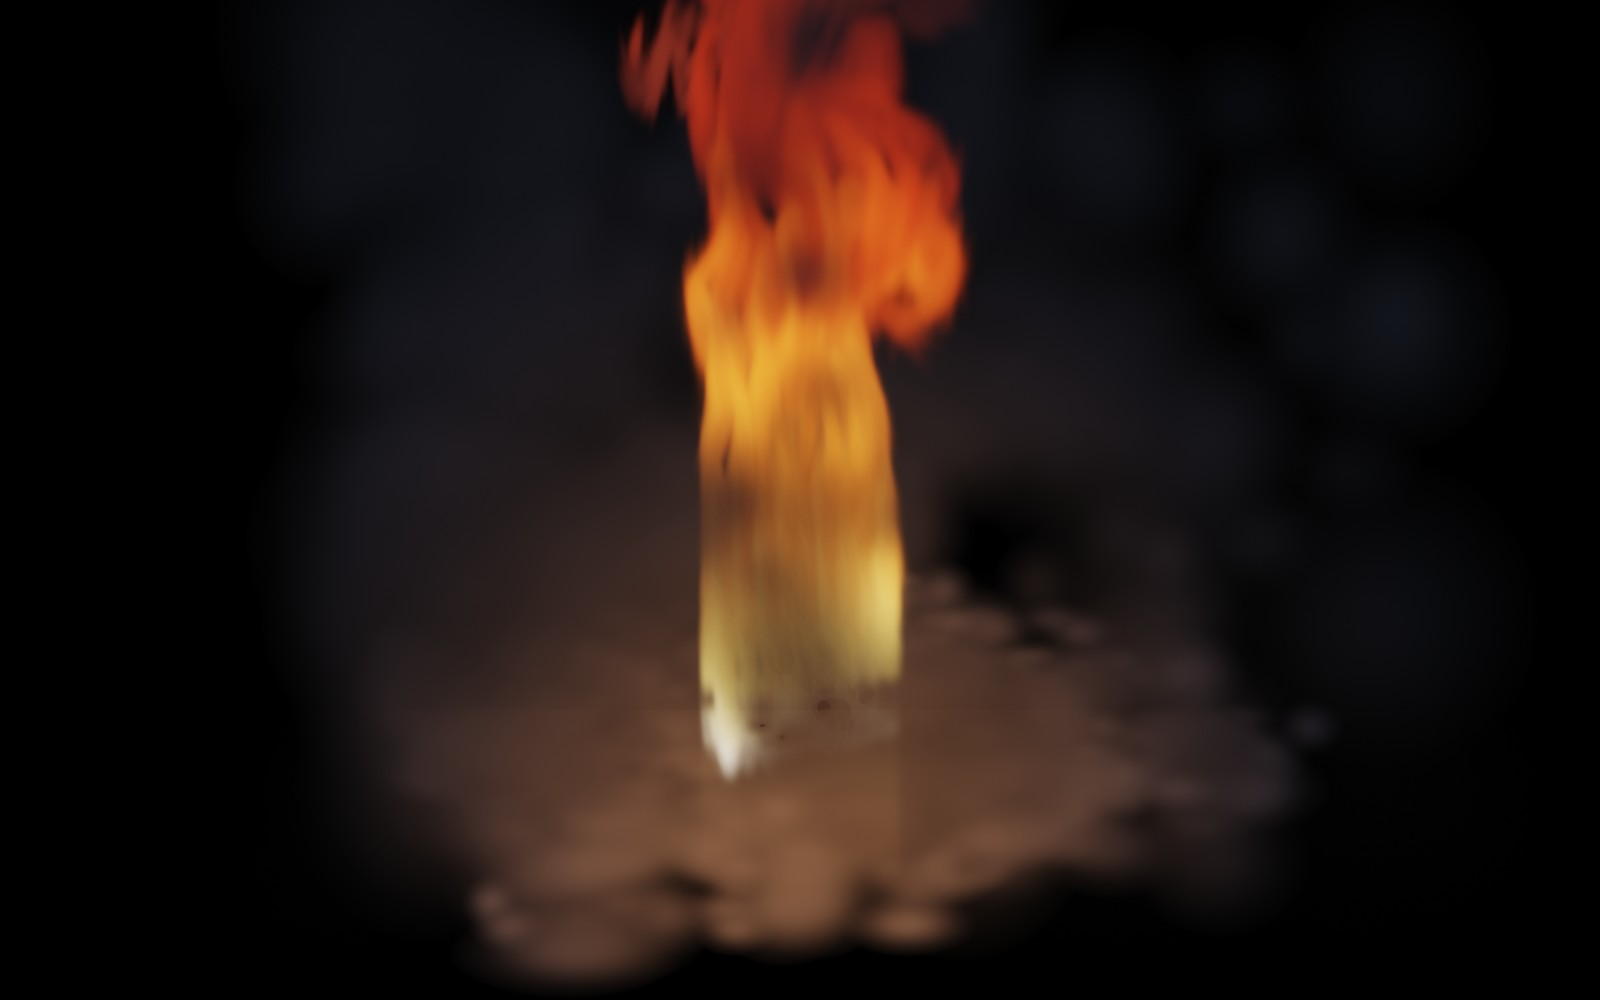
\includegraphics[width=.492\linewidth]{interz_on}\\[2pt]
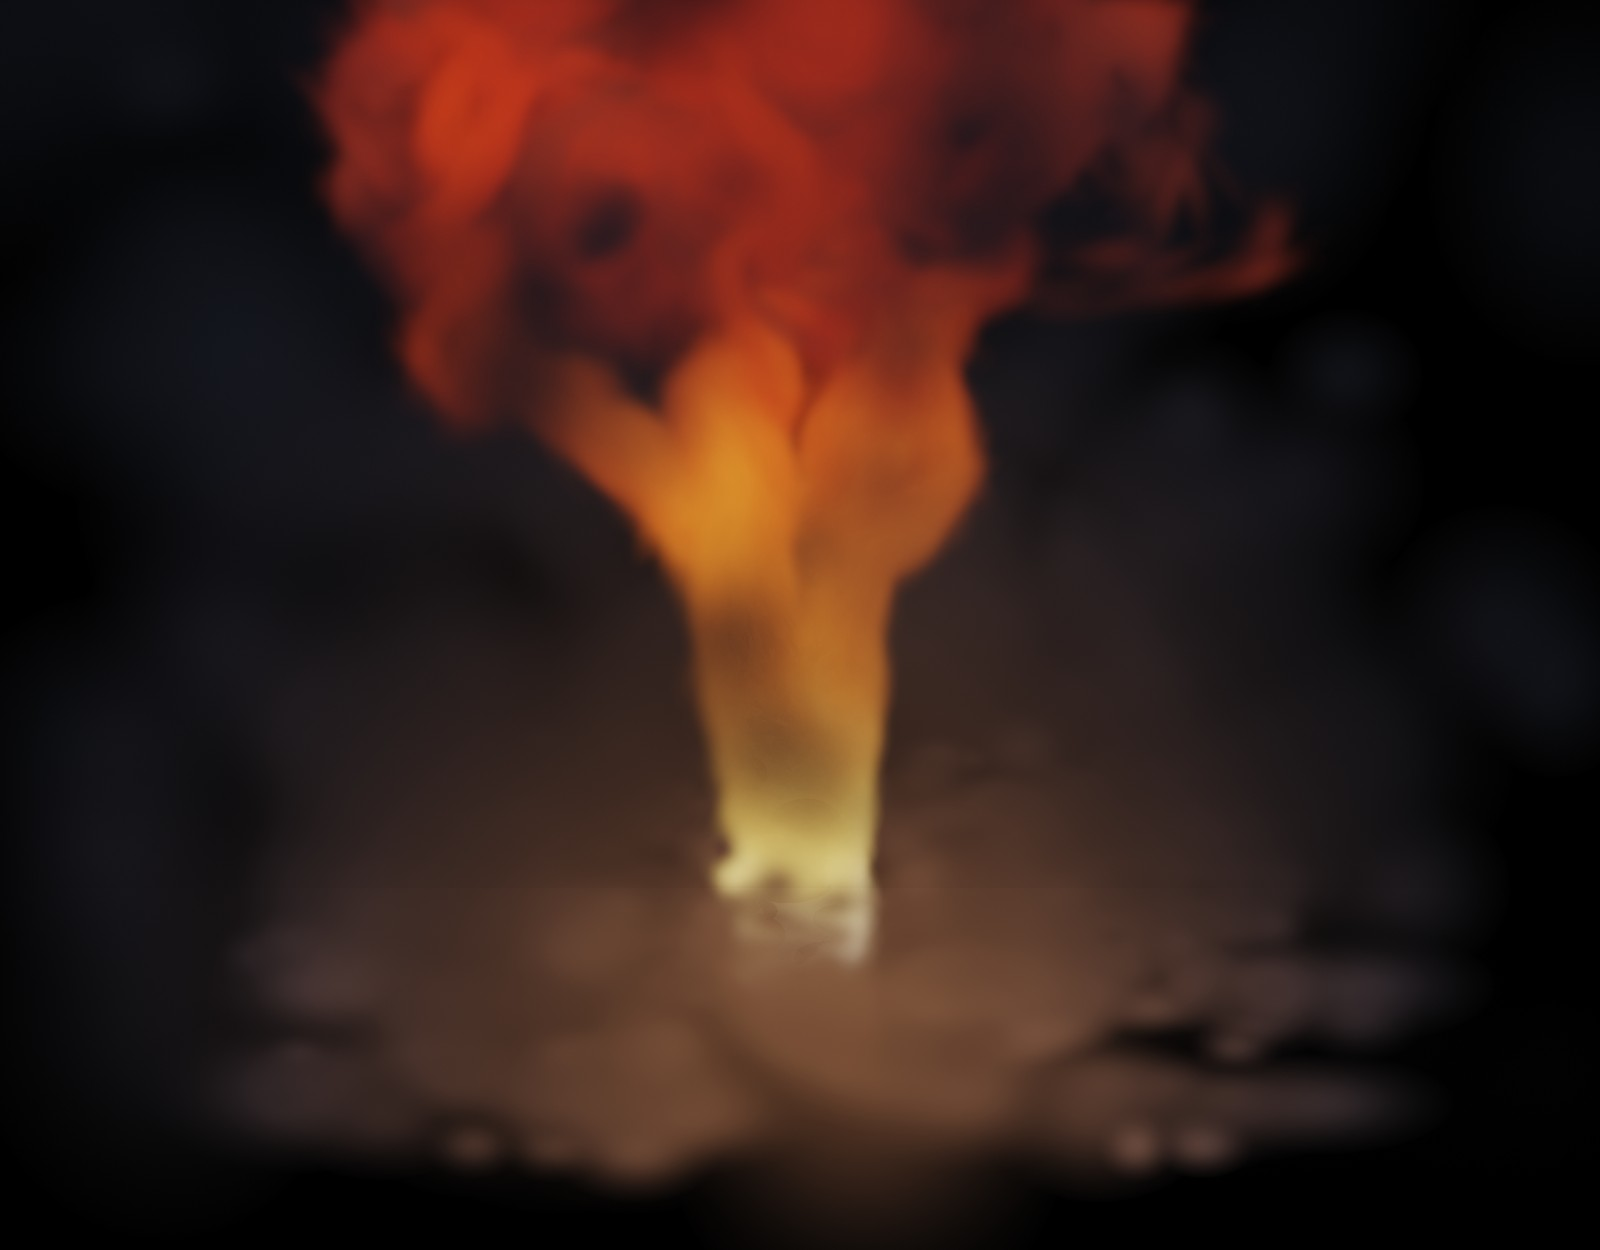
\includegraphics[width=.492\linewidth]{bloom_a}\hfill
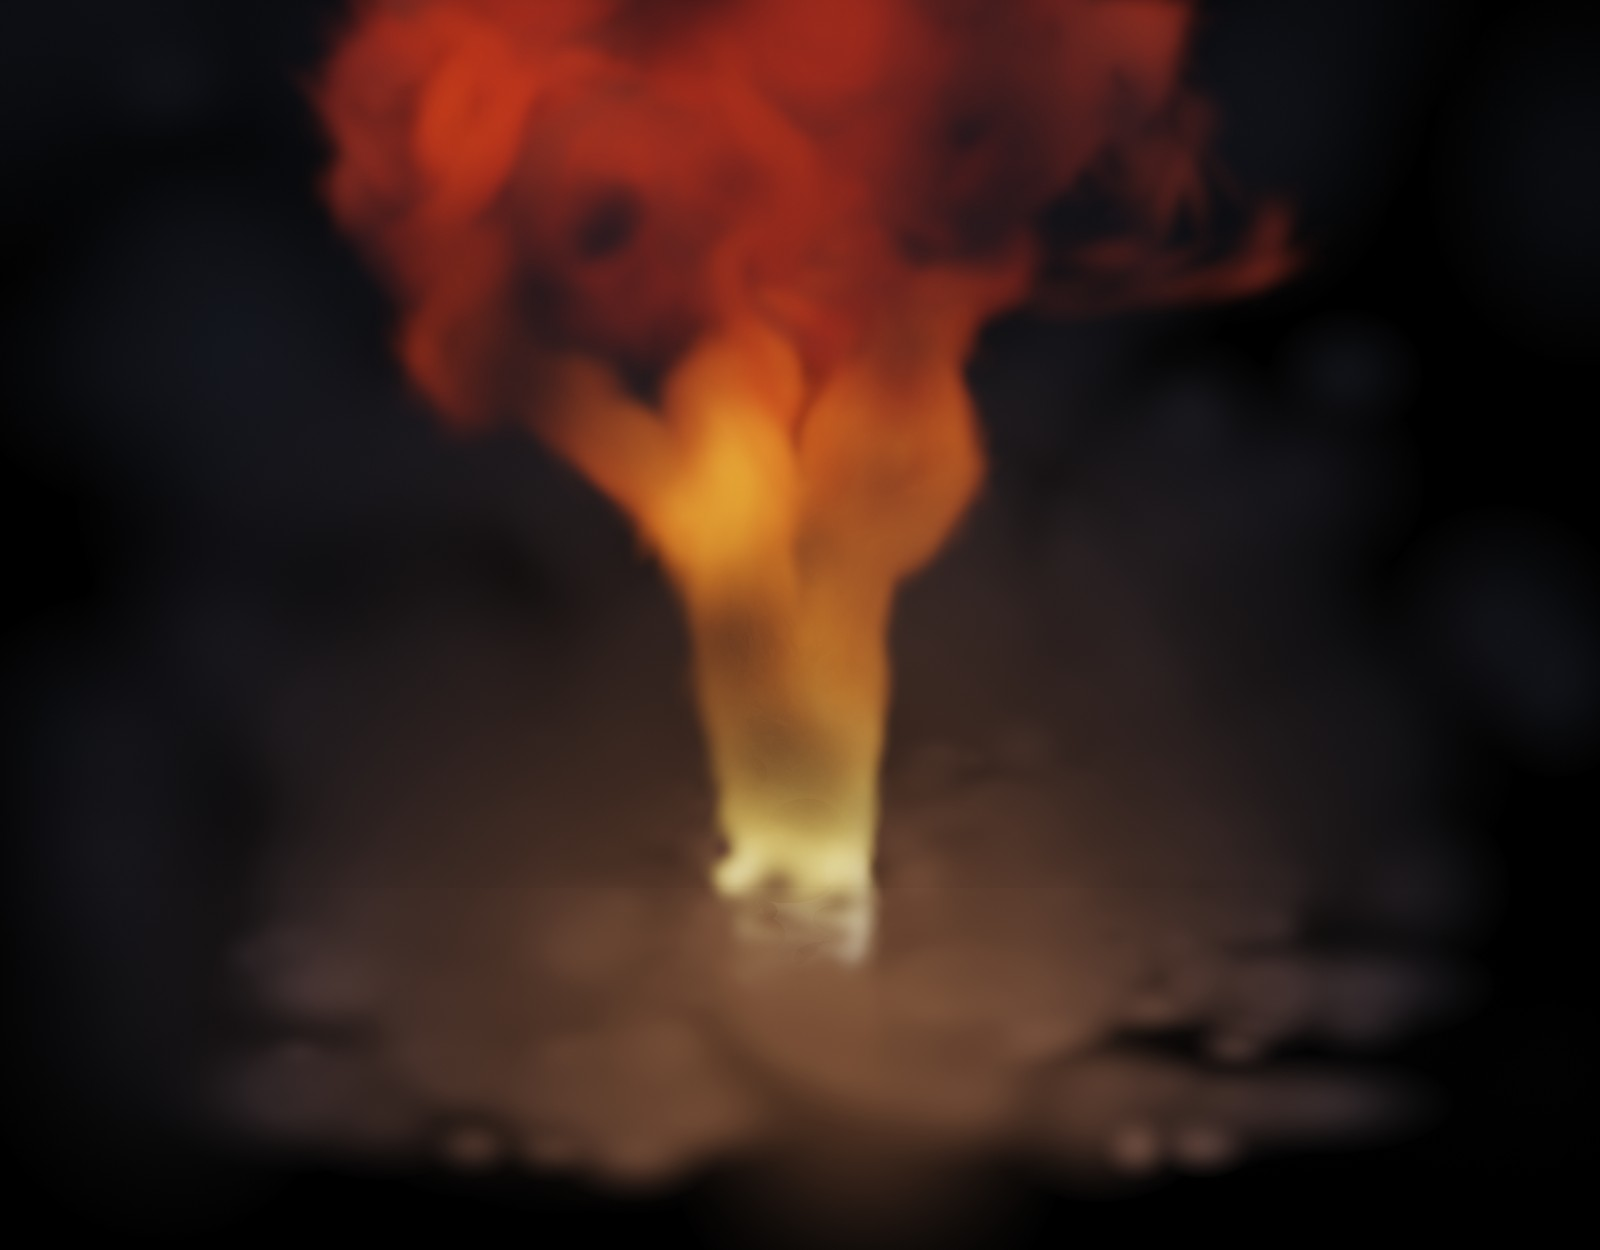
\includegraphics[width=.492\linewidth]{bloom_b}
\caption{Rows: procedural source, then simulated; view-aligned slices, then world-fixed at a $79^\circ$ orbit; $\kappa_z=0$, then 0.45 at a $63^\circ$ side view; without and with bloom. Within a pair the seed, step count, camera and shading are identical.}
\end{figure}

\begin{figure}
\centering
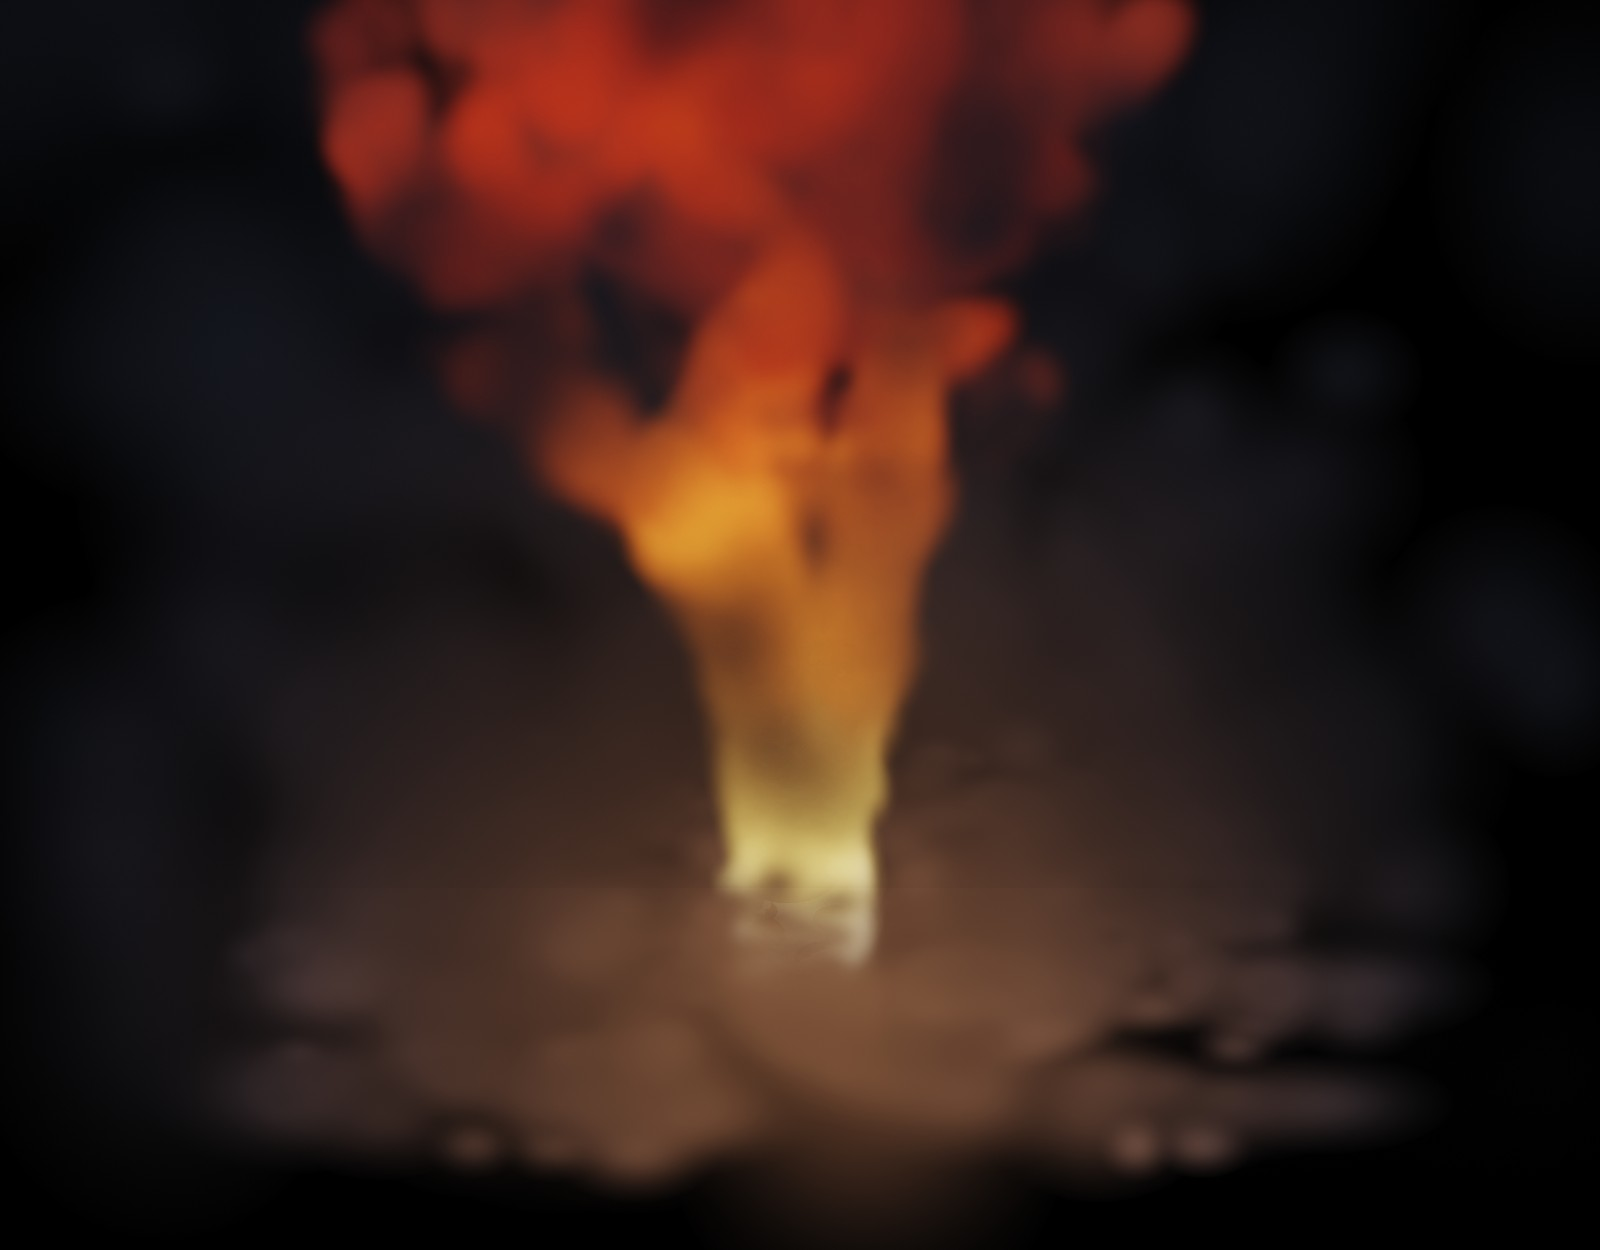
\includegraphics[width=.325\linewidth]{cov_a}\hfill
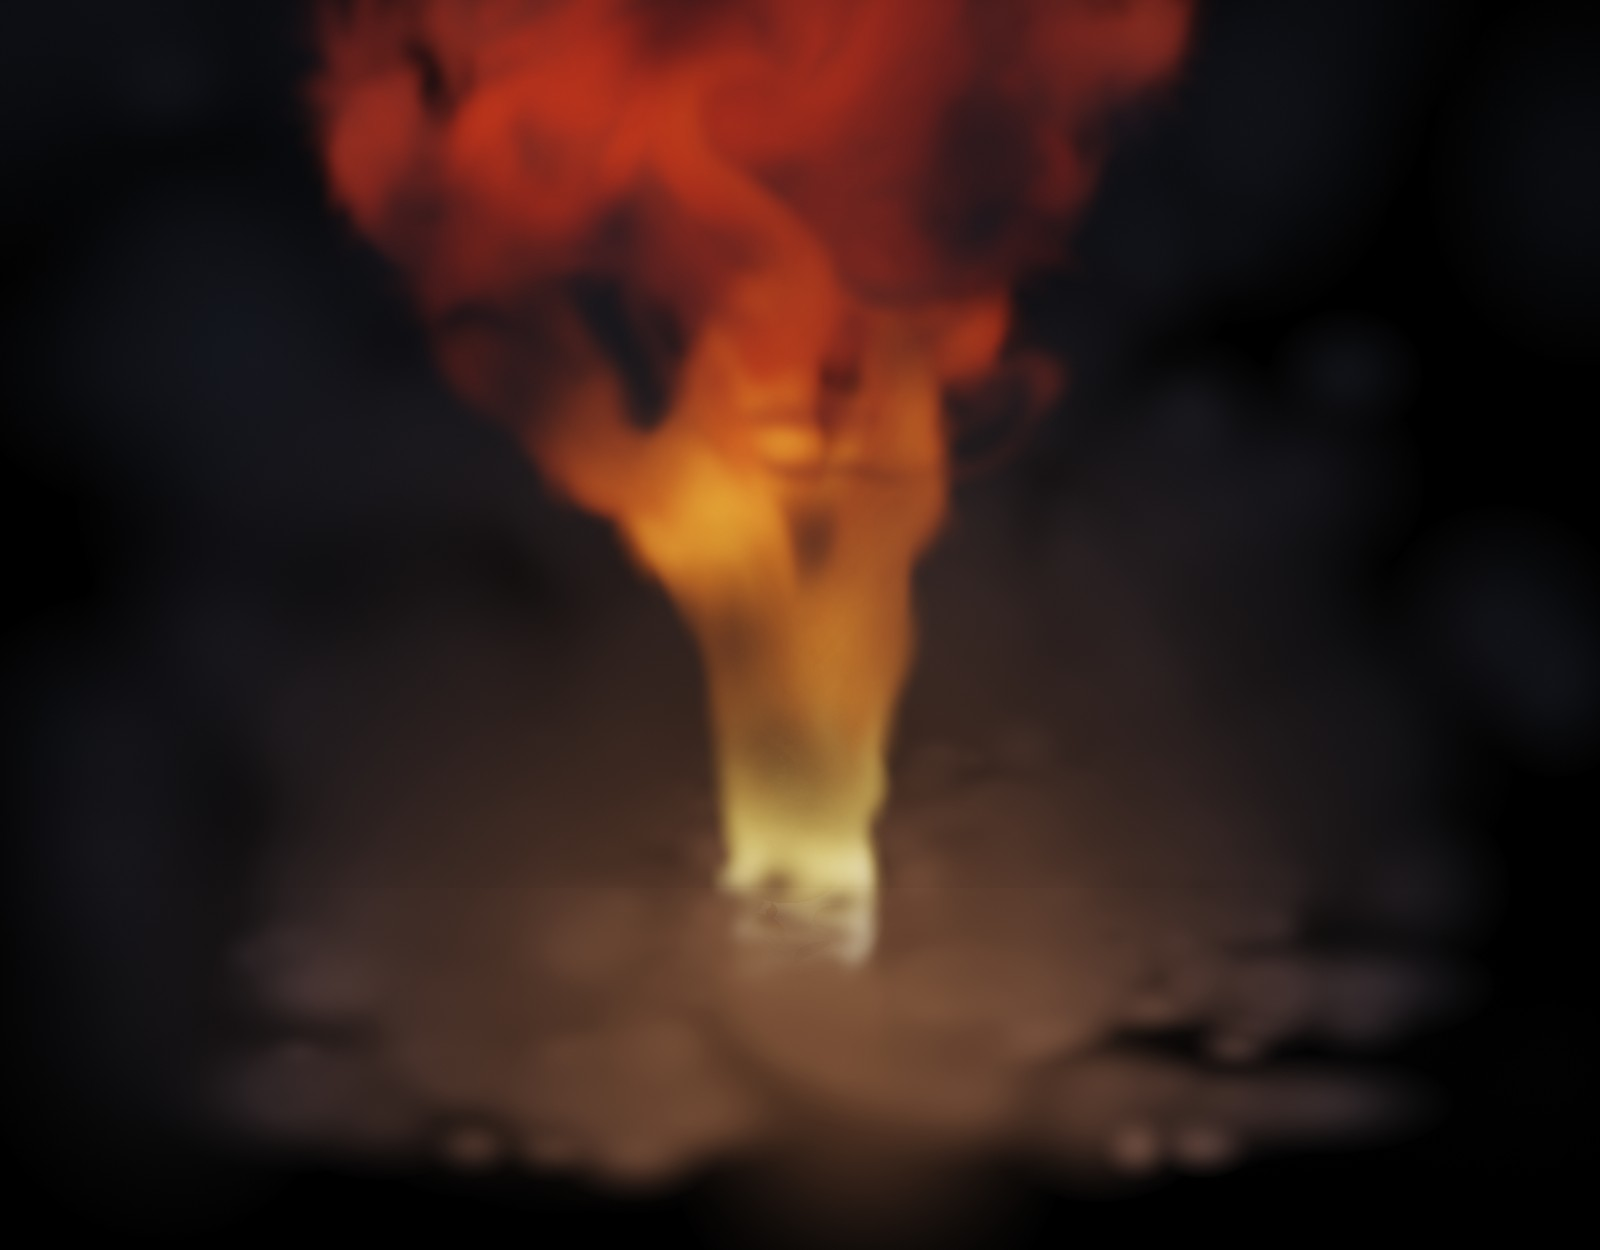
\includegraphics[width=.325\linewidth]{cov_b}\hfill

\includegraphics[width=.325\linewidth]{cov_c}\\[4pt]
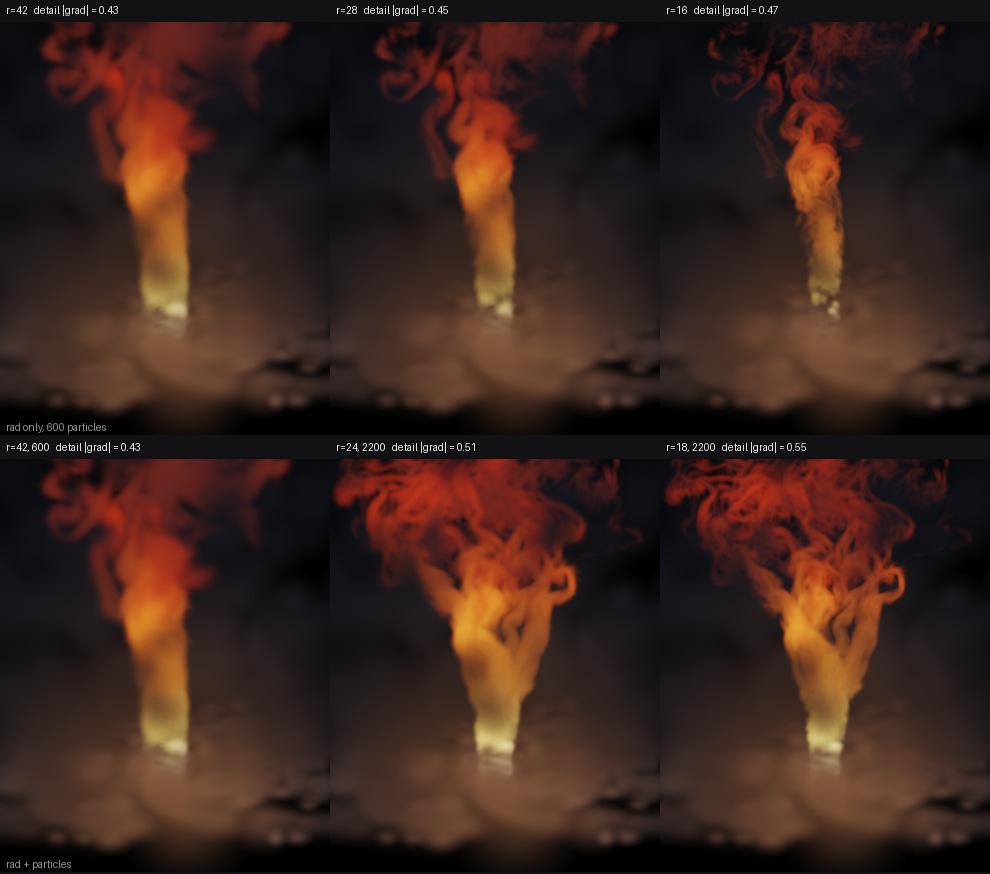
\includegraphics[width=.75\linewidth]{radius}
\caption{Top: isotropic splats, flow-driven covariance, and trajectory filaments. Bottom: perceived detail is bounded by the particle budget. Mean image gradient rises 0.43 to 0.47 from radius 42 to 16 at 600 particles per layer, but below $\sim$22 the blobs stop tiling; 2200 particles reach 0.51 at radius 24 and 0.55 at 18.}
\end{figure}

\section{Solver pseudocode}
\begin{lstlisting}
step_all(dt):                       # once per frame
  for each sim layer L:             # emit + pack + build
    emit at source (budgeted)
    for particle i in L:
      if in source band: T_i += dt*s0*exp(-ks*x~^2)
      T_i *= (1 - 0.5*kc*dt); clamp
      if nu > 0: sig_i^2 += 2*nu*dt
    Morton-sort; pack SoA in sorted order
    build quadtree; per node: signed Gamma,
      |Gamma|-centroid, signed dipole, matched sig_c^2
  director = merge top levels across layers
             + ground images (x,-y,-Gamma)
  circles  = cut sphere proxies by each slice
  if kz > 0: pairwise exchange between adjacent layers
step_slice(L, dt):                  # N-body + update
  for particle i:
    traverse tree once, accumulating in closed form:
      u_i, grad-u L_i, sum w, sum w*T, dT/dx moments
    v = u_i + beta_b*T~ * y-hat
    v += c*(U_director(x_i) - v)
    v += turb*curl_noise(x_i,t) + wind
    for each nearby circle: v += doublet; wall layer
    clamp |v|
  for particle i:
    G_i = (1-lam*dt)*G_i + dt*(beta*dTdx_i + wall_i)
    Sigma_i evolved by L_i
    x_i += dt*v_i; push out of circles
    Tc_i -= dt*kappa*Tc_i^2; d_i *= (1 - 0.3*dt)
    recycle if cold/exhausted/out of bounds
render():
  gather and sort particles; bin into six light clusters
  bucket scene splats; interleave streams front to back
\end{lstlisting}

\section{Videos}
\paragraph{Main video.} 95\,s, seven single-take sequences on the shipping $9\times600$ configuration at fixed $\Delta t=1/60$\,s, so playback speed equals simulation speed. Three side-by-side sequences compare the vortex-in-cell baseline and the grid-free solver from one seed. Overlay rates are the fire alone (15.5\,ms grid, 17.1\,ms grid-free). The sequences inside the loaded synthetic scene run at 36.4\,ms end to end.

\paragraph{Hero clips.} 6\,s at $1920\times1080$, 60\,fps: the fire alone and the fire in the synthetic scene under world-space light, both at the Hero preset. These are offline renders with one fixed step per frame.

\paragraph{Captured scene and Omniverse clips.} The kitchen clip is an offline orbit of the loop on \emph{kitchen}. The Omniverse clip is the farmland render of the main paper's \S7.7: 8\,362\,588 Gaussians in the capture and a full-density crop of 1\,892\,830 static surroundings plus 736\,360 farmhouse splats, 15\,s at two fixed $\Delta t=1/60$\,s steps per output frame at 30\,fps.

\paragraph{Reproduction.} \texttt{tools/harness.py} reproduces the hash anchors, GPU-synchronized timings, deflection statistics and the Hero stills. \texttt{study/analyze.py} is the pre-registered analysis.

\bibliographystyle{ACM-Reference-Format}
\input{refs_supp.bbl}
\end{document}
